\documentclass[10pt,journal,compsoc]{IEEEtran}
\usepackage{graphicx}
\usepackage{float}
\usepackage{algorithm}
\usepackage{algorithmic}
%\usepackage{algpseudocode}
\usepackage{tabularx}
\usepackage{tabularx}
\usepackage{chemarrow}
\usepackage{amsmath}
\usepackage{amsthm}
\usepackage{enumerate}
\usepackage{boxedminipage}
\usepackage[normal]{caption}
\usepackage{amsmath}
\usepackage{amsfonts}
\usepackage{multirow}
\usepackage{xspace}
\usepackage{textcomp}
\usepackage{amssymb}
\usepackage{url}
\usepackage[usenames,dvipsnames]{color}
\usepackage{xcolor}
\usepackage[OT1]{fontenc}

%\geometry{left=1 in,right=1 in,top=1 in,bottom=1in}


\ifCLASSOPTIONcompsoc
  \usepackage[caption=false,font=normalsize,labelfont=sf,textfont=sf]{subfig}
  \usepackage{cite}
\else
  \usepackage[caption=false,font=footnotesize]{subfig}
  \usepackage{cite}
\fi

\renewcommand{\algorithmicrequire}{\textbf{Input:}}
\renewcommand{\algorithmicensure}{\textbf{Output:}}
\renewcommand\arraystretch{1.5}
\newcommand{\tabincell}[2]{\begin{tabular}{@{}#1@{}}#2\end{tabular}}

\newcommand{\ours}{\ensuremath{\tt DV}\xspace}

\newcommand{\algorithmicbreak}{\textbf{break}}
\newcommand{\BREAK}{\STATE \algorithmicbreak}
\graphicspath{{fig/}}

\theoremstyle{plain}
\newtheorem{theorem}{Theorem}

\theoremstyle{definition}
\newtheorem{definition}{Definition}

\newcommand{\name}{\ensuremath{{\tt GSSE}}\xspace}
\newcommand{\mdsse}{\ensuremath{{\tt MDSSE}}\xspace}
\newcommand{\blue}{\textcolor{blue}}
\newcommand{\red}{\textcolor{red}}

\hyphenation{op-tical net-works semi-conduc-tor}


\begin{document}

%\title{A Verifiable Dynamic Scheme based on Multi-User Symmetric Searchable Encryption}
%\title{A Generic Verifiable Symmetric Searchable Encryption With Flexible Updates }
%\title{Enabling Verifiable, Dynamic, and Multi-User Symmetric Searchable Encryption}
\title{\blue{Enabling Generic, Verifiable, and Secure Data Search in Cloud Services}}
%Dynamic Scheme based on Multi-User Symmetric Searchable Encryption}

\author{Jie Zhu, Qi Li,~\IEEEmembership{Senior Member, IEEE}, Cong Wang,~\IEEEmembership{\red{Senior} Member, IEEE}, Xingliang Yuan,~\IEEEmembership{Member, IEEE}, \\ Qian Wang,~\IEEEmembership{Member, IEEE}, Kui Ren,~\IEEEmembership{Fellow, IEEE}
\IEEEcompsocitemizethanks{\IEEEcompsocthanksitem J. Zhu and Q. Li are with Graduate School at Shenzhen, Tsinghua University, Shenzhen, China, and Dept. of Computer Science, Tsinghua University, Beijing, China. \protect E-mail: j-zhu15@mails.tsinghua.edu.cn, qi.li@sz.tsinghua.edu.cn. \protect
\IEEEcompsocthanksitem C. Wang is with Dept. of Computer Science, City University of Hong Kong, Hong Kong. \protect E-mail: congwang@cityu.edu.hk. \protect
	\IEEEcompsocthanksitem \red{X. Yuan is with Faculty of Information Technology, Monash University, Australia.} \protect \red{E-mail: xingliang.yuan@monash.edu.} \protect
    \IEEEcompsocthanksitem Q. Wang is with School of Computer Science, Wuhan University, \blue{Wuhan}, China. \protect E-mail: qianwang@whu.edu.cn. \protect
	\IEEEcompsocthanksitem K. Ren is with Institute of Cyber Security Research, Zhejiang University, China. \protect
	E-mail: kuiren@zju.edu.cn.
}}

\IEEEcompsoctitleabstractindextext{
\begin{abstract}
% Cloud storage enables users to manage and share their data at low cost, but it also introduces data security issues. 
\red{Searchable Symmetric Encryption (SSE) has been widely studied in cloud storage, which allows cloud services to directly search over encrypted data. Most SSE schemes only work with honest-but-curious cloud services that do not deviate from the prescribed protocols. However, this assumption does not always hold in practice due to the untrusted nature in storage outsourcing. To alleviate the issue, there have been studies on Verifiable Searchable Symmetric Encryption (VSSE), which functions against malicious cloud services by enabling results verification. But to our best knowledge, existing VSSE schemes exhibit very limited applicability, such as only supporting static database, demanding specific SSE constructions, or only working in the single-user model. In this paper, we propose GSSE, the first generic verifiable SSE scheme in the single-owner multiple-user model, which provides verifiability for any SSE schemes and further supports data updates. To generically support result verification, we first decouple the proof index in GSSE from SSE. We then leverage Merkle Patricia Tree (MPT) and Incremental Hash to build the proof index with data update support. We also develop a timestamp-chain for data freshness maintenance across multiple users. Rigorous analysis and experimental evaluations show that GSSE is secure and introduces small overhead for result verification.}
% \red{In the context of cloud storage, searchable symmetric encryption (SSE) has been widely studied, which allows cloud services to directly search over encrypted data. Despite promising, most SSE schemes only work with honest-but-curious cloud services that do not deviate from the prescribed protocols. This assumption, however, does not always hold in practice due to the untrusted nature in storage outsourcing. To alleviate the issue, there have been studies on Verifiable Searchable Symmetric Encryption (VSSE), which functions against malicious cloud services by enabling search results verification. But to our best knowledge, existing VSSE schemes exhibit only very limited applicability, such as supporting static database at best, demanding specific searchable encryption constructions, or only working in the single-user model. In this paper, we propose GSSE, the first generic verifiable SSE scheme in the single-owner multiple-user model, which provides verifiability for any existing SSE schemes and further supports data updates. To generically support result verification, we first decouple the proof index generation in GSSE from SSE operations. We then leverage Merkle Patricia Tree (MPT) and Incremental Hash to carefully build the generic proof index with data update support. To prevent replay attacks, we further develop a timestamp-chain for the data freshness maintenance across multiple users. Through rigorous analysis and experimental evaluations, we show GSSE is secure and introduces small extra overhead for result verification.}

\end{abstract}


%However, most of the existing VSSE schemes focus on single-user setting. But in fact, known cloud services also support data sharing among the users.

% against a malicious server
}
\maketitle
\section{Introduction}
\blue{\red{Cloud storage allows users to retrieve and share their data conveniently with well understood benefits, such as on-demand access, reduced data maintenance cost, and service elasticity~\cite{juels2007pors,ateniese2008scalable,kamara2011cs2,wang2011enabling,stefanov2012iris,kamara2013parallel,sun2015catch}. Meanwhile}, cloud storage also brings serious data privacy issues, i.e., the \blue{disclosure of private information}.
In order to ensure data privacy without losing data usability, a cryptographic notion named searchable symmetric encryption (SSE), \red{(e.g., \cite{song2000practical,curtmola2011searchable,kamara2012dynamic,cash2014dynamic,wang2016searchable}, to just list a few)}, has been proposed. \blue{By using SSE, users \red{can} encrypt their data before uploading to cloud services, and cloud services can directly operate and search over encrypted data, which ensures data privacy.}}

\blue{However, most existing SSE schemes~\cite{curtmola2011searchable, kamara2012dynamic, cash2014dynamic} are built based on the assumption that cloud services are honest but curious, which means cloud services will follow the protocol but intend to derive users' information from their search queries. \red{Unfortunately, this assumption does not always hold in practice, since cloud services may be subject to external attacks, internal misconfiguration errors, software bugs, and even insider threats~\cite{sun2015catch,bost2016verifiable}. All these factors may cause the cloud services to deviate from the prescribed protocol and operate beyond the honest-but-curious model. Exemplary consequences might be cloud services executing a fraction of search operations or omitting some files in search results.}}



\begin{table*}[t]
  \begin{center}
  \caption{Comparison with existing typical verifiable SSE schemes.}
  \label{tab:comparison}
  %\begin{threeparttable}
  \begin{tabular}{|c|c|c|c|c|c|c|c}
    \hline
                                          &\blue{Dynamism}     &Three-party$^1$    &Freshness Verify$^2$     &Integrity Verify$^3$    & \blue{Prove Efficiency}$^4$        &Generality$^5$  \\
    \hline
    \hline
    KPR11~\cite{kamara2011cs2}            &\checkmark     &\texttimes     &\checkmark         &\texttimes                          &$O(|W|)$                      &\checkmark  \\
    \hline
    KO12~\cite{kurosawa2012uc}            &\texttimes     &\texttimes     &\text{-}           &\texttimes                          &$O(n)$                        &\texttimes\\
    \hline
    CG12~\cite{chai2012verifiable}        &\texttimes     &\texttimes     &\text{-}           &\checkmark                          &$O(log(|W|))$                 &\texttimes  \\
    \hline
    KO13~\cite{kurosawa2013update}        &\checkmark     &\texttimes     &\checkmark         &\texttimes                          &$O(n)$                        &\texttimes \\
    \hline
    SPS14~\cite{stefanov2014practical}    &\checkmark     &\texttimes     &\checkmark         &\texttimes                          &$min\{\alpha + log(N), r log^3(N)\}$                  &\texttimes \\
    \hline
    CYGZR15\cite{cheng2015verifiable}    &\texttimes     &\texttimes      &\text{-}         &\texttimes                            &$O(|W|)+O(r)$                 &\texttimes \\
    \hline
    BFP16~\cite{bost2016verifiable}       &\checkmark     &\texttimes     &\checkmark         &\checkmark                          &$O(r)$                        &\checkmark   \\
    \hline
    OK16~\cite{ogataefficient}            &\texttimes     &\texttimes     &\text{-}           &\checkmark                          &$O(r)$                        &\checkmark  \\
    \hline
    \name                                 &\checkmark     &\checkmark     &\checkmark         &\checkmark                          &$O(log(|W|))$                 &\checkmark  \\
    \hline
  \end{tabular}\\
  \end{center}
  $^1$ Three-party means whether the scheme supports search result verification for an SSE scheme with three parties, i.e., data owners, servers, and users.\\
  $^2$ Note that, '\texttimes' represents the requirements which are not implemented, while '-' means the requirements which are not required. Specifically, the static verifiable SSE schemes do not have the problem of data freshness attacks, and thus the existing schemes~\cite{kurosawa2012uc,chai2012verifiable,cheng2015verifiable,ogataefficient} do not require data freshness verification.\\
  $^3$ We consider various data integrity attacks, especially the attacks that servers can intentionally returns an empty result to evade search result verification.\\
  $^4$ \red{The prove efficiency refers to the cost of operations for search result verification. For some selected non-generic schemes~\cite{kurosawa2012uc,chai2012verifiable,kurosawa2013update,stefanov2014practical,cheng2015verifiable}, their prove efficiency is equivalent to their encrypted search efficiency. Here, $n$ indicates the number of total files, $|W|$ means the number of all keywords, $r$ means the number of files which contain the specific keyword, $\alpha$ means the number of times this keyword was historically added to the collection \cite{stefanov2014practical}, and $N$ means the total number of document and keyword pairs.}\\
  $^5$ A generic VSSE scheme means that the verifiable design can provide result verification for any SSE schemes, while a non-generic scheme only works for a particular SSE construction.\\
\end{table*}


%{\bf There have been a lot of researches
\blue{In order to address this issue, a large amount of studies~\cite{wang2011enabling, zhu2012cooperative, juels2007pors, stefanov2012iris, ateniese2007provable, erway2015dynamic} have  been conducted to ensure data integrity against a malicious cloud server}. Also, verifiable SSE schemes  \cite{kamara2011cs2,kurosawa2012uc,chai2012verifiable,kurosawa2013update,stefanov2014practical,cheng2015verifiable,bost2016verifiable,ogataefficient} have been developed to ensure data integrity in SSE.
\blue{Unfortunately, these schemes either support verification on only static database~\cite{kurosawa2012uc,chai2012verifiable,cheng2015verifiable,ogataefficient}, or cannot prevent cloud services from deliberately returning an empty result to evade result verification~\cite{kamara2011cs2,kurosawa2013update,stefanov2014practical}.}
Specifically, \red{previous schemes that are} built on Merkle Hash Tree~\cite{kamara2011cs2}, RSA accumulator~\cite{kurosawa2013update}, or Message Authenticated Code (MAC)~\cite{stefanov2014practical} \red{are not able to} return any search result when there does not exist any document matching the query keywords~\cite{bost2016verifiable}. To prevent the server from returning an empty result maliciously, the user should maintain all keywords of the data set locally. Recently, Ogata et al. \cite{ogataefficient} addressed the issue by maintaining keywords with a cuckoo hash table. Unfortunately, the scheme cannot enable verification under data updates.
\red{Further, most} verifiable SSE schemes~\cite{kamara2011cs2,kurosawa2012uc,chai2012verifiable,kurosawa2013update,stefanov2014practical,
cheng2015verifiable,ogataefficient,bost2016verifiable} only enable verifiability for the single-user model, \red{which we refer to as the two-party model}. However, in practice, service providers such as public cloud normally enable data sharing among \red{the data owner and multiple data users} in a three-party model, where data owner and user are not the same entity. Table~\ref{tab:comparison} compares various existing verifiable SSE schemes. \red{To our best knowledge,} none of the existing verifiable SSE schemes can explicitly allow users to verify their search results \red{in} the three-party model.
%, i.e., data users separate from the data owners.


%In particular, they cannot prevent the data integrity attacks, e.g., clouds may deliberately omit search results, and the replay attacks, e.g., clouds can replay the previous results. The problems above motivate us to revisit SSE.
% and  design a generic dynamic verifiable SSE
% schemes in the multi-user scenario which not only support the result verification against the data integrity attack, but also support the preventing of the replay attack.
In this paper, we propose \name, a generic dynamic verifiable SSE framework to ensure \red{search result} integrity and freshness across multiple users. It can be applied to any SSE schemes, \red{including but not limited to those in~\cite{stefanov2014practical,cash2014dynamic,kamara2012dynamic}, etc., to provide search results verification for data users. In addition, it supports data updates, a highly desirable advantage demanded by many modern cloud storage applications, where data update happens frequently.} %It is the first generic and verifiable SSE, which can be applied to various existing SSE schemes~\cite{stefanov2014practical,cash2014dynamic,kamara2012dynamic} while enabling verifiability across multiple users.}

\name addresses two challenges in verifying search results of SSE. The first challenge is how to design an efficient yet \red{generic} proof index which not only supports data integrity verification but also supports data updating. \name builds and maintains such a proof index by \red{leveraging the fully dynamic and balanced Merkle Patricia Tree (MPT)~\cite{merkle_patricia_tree} and Incremental Hash~\cite{bellare1994incremental}. With these two prelimitives,} we store encrypted keywords and their corresponding documents in the proof index such that the root of the MPT becomes an accumulator of the data\red{,} which can be treated as a witness of data integrity. Meanwhile, \name designs a verification mechanism based on the proof index to ensure the authenticity of search results. \blue{Different from the previous solutions~\cite{kamara2011cs2,kurosawa2013update,stefanov2014practical}, our scheme requires the server to return a proof to the users regardless of whether the keyword exists or not, such that the users can detect whether the cloud services deliberately omit all files and returning an empty result to evade result verification.} More specially, \name does not require the users to maintain a large set of keywords, while easily verifying the integrity of the search results with the proof.

The second challenge is how to ensure data freshness by preventing the root from being replayed \red{in the context of data updates}. In the previous two-party model, \red{data ower} can recalculate the root after each update, but \red{in} the three-party model, data users cannot easily detect a data update \red{from} the data owner\red{, unless} data owner sends the latest root to \red{all users} after each data update. \red{But doing so would bring in significant, if not impractical, online communication burden to the data owner}.
In order to solve this problem, we develop a timestamp-chain based verification mechanism for \name. This mechanism constructs a timestamp-chain based authenticator which \red{includes} the root of the MPT. \blue{It allows users to obtain an authenticator from cloud services on demand and easily ensure the freshness of the root while not incurring significant computation and communication overhead.}
%To address our challenges, our first obstacle is how to design an efficient proof index and meanwhile prevent the server from evading the result verification. \name builds and maintains an efficient proof index by leveraging the Merkle Patricia Tree (MPT). We store encrypted keywords and their corresponding documents in the proof index such that \name enables search over encrypted keywords, and ensures the authenticity of search results under data insertions and deletions. \name allows users to verify their search results according to the proofs presented by the cloud servers such that the users can detect whether the clouds deliberately omit some files from the search results, specially, omitting all files and returning an empty result to evade result verification. Therefore, users can easily validate the integrity of the search result.
%
%Moreover, in order to prevent search results and the corresponding proofs from the replay attacks, we develop a timestamp chain based verification mechanism for \name. This mechanism constructs a timestamp chain for all authenticators that include the proofs of updated data and the update timestamp. Therefore, it allows users to obtain an authenticator from the cloud server on demand and compare it with that stored in the timestamp chain computed by the users. Therefore, the users can easily ensure the correctness of the proofs and detect the replay attacks in realtime if the two authenticators are different, while not incurring significant computation and communication overhead.
%
%The reasons that the existing verifiable SSE schemes for the three-party model cannot ensure the integrity of search results are two-fold. Firstly, users cannot easily synchronize with the data owners if the dataset of a data owner is dynamic. Thereby, users cannot detect a replay attack if the clouds return the previous search results. Secondly, a cloud can simply tamper with the search results and return the modified results to the users. In particular, it can completely omit all search results so as to evade the verification of the existing verifiable SSE scheme.%, even though a timestamp is applied.
%
%Recent work by Kurosawa et.al. \cite{kurosawa2012uc} first proposed the concept of verifiable SSE (VSSE) and extend it to a dynamic solution \cite{kurosawa2013update}. Generally speaking, there are two main types of attacks in the VSSE problem, one is the \textit{replay attack} which means the cloud intends to return the old version of the data to the user (e.g., data before adding, deleting or editing) and the other is the \textit{data integrity attack} which means the cloud intends to omit some files or even omit all the files to save its computation costs or download bandwidth. Most of the exiting solutions do not consider the situation when the cloud omits all the files except the generic VSSE schemes proposed by Bost et.al. \cite{bost2016verifiable}, but their scheme need two communication round between the cloud and the user. And unfortunately, all of the above schemes are established under the two-party model, e.g. the client-server model. To the best of our knowledge, there are no research address the VSSE problem in a multi-user model, because it is much more complicated to prevent the replay attack in the multi-user scenario.
%
%To address the challenges, our first obstacle is how to design an effient proof index for result verification. Here, we leverage the MPT which is balance of the Merkle Tree and the Trie Tree. This structure enables the search of the encrypted keyword and meanwhile ensure the authentication capability and is fully dynamic for data insertions and deletions. Specifically, we store the encrypted keyword and its corresponding documents in this proof index and design a prove algorithm excuted by the cloud for the following checking of the data integrity. The proof produced by the prove algorithm not only enables the data user to verify the search result when the cloud omits some files, but also allows the user to verify the search results when the cloud deliberately return an empty file set.
%
%Our second obstacle is how to prevent the replay attack launched by the cloud. Since the cloud is untrusted, the data user can only trust the data owner when there is no trusted authority. Consider the following two models: First, the push model, e.g., the data owner broadcasting the proof to every user after each update. Second, the pull model, e.g., the data user retrieve the proof from the data owner when he need. However, both of the above models require frequent interaction between the data owner and the data user, and the communication cost becomes larger when the update frequency increases and the number of users grows. We propose a new chained-timestamp solution which allows the users to obtain the result proof from the cloud on demand and meanwhile does not introduce significant overhead to the data owner.
%
In summary, our contributions are three-fold:
\begin{enumerate}
  \item \red{We propose the first generic verifiable SSE framework, i.e., \name, in the single-owner multiple-user model, which provides verifiability for any existing SSE schemes and further supports data updates.}
  %based on the multi-user scenario which enables the users to check the data integrity over the search result while providing a detection mechanism against the repaly attack.
  \item We develop verification mechanisms for \name such that it can ensure both the freshness and integrity of search results across multiple users and data owners. \red{Rigorous analysis formally shows the security strength of \name.}

  %We propose a fully dynamic Verifiable scheme leverage the Merkle Patricia Tree, and carefully tailor our design with detailed protocol illustration.
  %\item We design a prove algorithm against the data integrity attack which can detects the malicious situation where the cloud tries to omit some files or even all the files.
  %\item We design a chained-timestamp machanism against the replay attack in the multi-user scenario.
  %\item experient and performance.
  \item \red{Through comprehensive experimental results, we show that \name only introduces small extra overhead for result verification, compared to existing searchable encryption schemes.}
\end{enumerate}

\section{Related Work}
\noindent\textbf{Secure Cloud Storage Scheme.} Verifiable cloud storage services have been extensively studied, e.g., Proof of Data Possession (PDP) \cite{ateniese2007provable, ateniese2008scalable, erway2015dynamic,zhu2012cooperative} and Proof \red{of} Retrievability (POR) \cite{juels2007pors, bowers2009proofs, stefanov2012iris}. \blue{These schemes mainly focused on verifying the integrity of data stored in cloud services and enable restoring data blocks if they are corrupted.} However, they did not ensure \red{the} integrity of search results,  \red{which is the focus of VSSE}.
Authenticated data structures are used by a set of searching algorithms to verify the integrity of data blocks stored on an untrusted server. Several schemes have been proposed, e.g., Merkle Tree\cite{merkle1987digital}, authenticated hash table\cite{papamanthou2008authenticated}, and \red{authenticated} skip list\cite{pugh1990skip,goodrich2001implementation}. Merkle Tree is the most common structure used to verify data integrity. However, Merkle Tree cannot flexible support data update. %is not a balanced tree when new leaf nodes are added and the searching operations are efficient.
Moreover, the current verification scheme~\cite{kamara2011cs2} built upon Merkle Tree did not store keyword information in its intermediate node and thus it is not suitable for keyword related searches. An authenticated hash table enabled by the RSA accumulator can be used to verify search results as well. Unfortunate, it has low efficiency in searching and update operations. For example, the search delay of the authenticated hash table is in millisecond level, while that of \name is in microsecond level. Skip list used a multilayer linked list to improve its search efficiency, but the storage overhead is much higher than a tree structure if the keyword information is required in the search path.
 %First, Merkle Tree is not a balanced data structure, and search delay of the authenticated hash table leveraging the RSA accumulator is lower than Merkle Patricia Tree. The search delay of the authenticated hash table is in millisecond level, while that of the authenticated hash table is in microsecond level. Second, the current Merkle Tree scheme proposed by Kamara et al. [5] did not store additional information such as keyword in its intermediate node, so that it cannot enable empty result validation

\noindent\textbf{Verifiable Searchable Symmetric Encryption.} The CS2 scheme \cite{kamara2011cs2} enabled users to verify the search result by using dynamic search authenticators, but their scheme cannot prevent the attacks that the server maliciously replies an empty result.
Recently Kurosawa et al.~\cite{kurosawa2012uc,kurosawa2013update,ogataefficient} proposed a few verifiable SSE schemes. However, their schemes either have low search efficiency, or do not support verification upon file update.
Kurosawa et al. \cite{kurosawa2012uc} required linear search in SSE and did not support dynamic file update. Their extension \cite{kurosawa2013update} achieved dynamic updating but the search complexity was beyond linear time. Recently, Ogata et al. \cite{ogataefficient} presented a generic verifiable scheme. It transforms any SSE scheme to a \textit{no-dictionary} verifiable SSE scheme that did not require the users to keep the keyword set. However, it was still a static approach, which shared the similar shortcoming with~\cite{chai2012verifiable} \cite{cheng2015verifiable}.
%Also, schemes in~\cite{chai2012verifiable} \cite{cheng2015verifiable} only enabled static SSE.
Although the verifiable scheme proposed by Stefanov et al.\cite{stefanov2014practical} achieved verifiability by leveraging message authenticated code, it cannot easily detect the data integrity attacks when the server intentionally returned an empty result.
Bost et al. \cite{bost2016verifiable} presented a generic verifiable dynamic SSE scheme and combined it with the SSE scheme proposed by Stefanov et al. \cite{stefanov2014practical}.
Yet, their scheme required two round communications for result verification and did not enable verification in the setting of multiple users. Our \name scheme is a generic verifiable SSE scheme that can work with three-party model, which can be \red{more readily} deployed in practice. In particular, it enables search result verification under file update with only one round of communication.


\noindent\textbf{Verifiable Public Key Encryption with Keyword Search.} The first verifiable attribute-based keyword search (VABKS) was proposed by Zheng et al. \cite{zheng2014vabks}. Similar to the existing SSE schemes above, VABKS only focused on search based on static encrypted data. Liu et.al \cite{liu2014efficient} proposed a more efficient construction based on VABKS, and Sun et.al \cite{sun2015catch} also provided a verifiable scheme VCKS that support conjunctive keyword search. However, due to the limitations of asymmetric encryption schemes, both of the above schemes require an additional trusted authority.


\noindent\textbf{Multi-User Searchable Encryption.} A few of non-verifiable multi-user schemes have been proposed~\cite{curtmola2011searchable,yang2009multiuser,jarecki2013outsourced,sun2016efficient}. Curtmola et al.~\cite{curtmola2011searchable} first proposed a multi-user SSE scheme based on broadcast encryption. Yang et al.~\cite{yang2009multiuser} proposed a multi-user searchable encryption scheme by leveraging a bilinear map. However, the search delay of the scheme is proportional to the size of the database, which is not suitable for large-scale databases.
Jarecki et al. \cite{jarecki2013outsourced} designed a multi-user scheme by using Oblivious Cross-Tags (OXT) protocol. However, their scheme required frequent communication between data owners and the users, which incured unnecessary communication overheads. Recently, Sun et al.~\cite{sun2016efficient} proposed a non-interactive multi-user searchable encryption schemes that reduced the interactions between data owner and users. However, the scheme did not support search under data update.

\section{Problem Statement}
\begin{figure*}[t]
\centering
\includegraphics[width=7 in]{mpt_detail}
\DeclareGraphicsExtensions.
\caption{The Merkle Patricia Tree}
\label{fig:mpt_detail}
\end{figure*}

In this section, we first formally define our problem and then present our design goals. We also review preliminaries used in this paper.



\subsection{Threat Model}
\blue{We assume that the data owner is trusted and the data users authorized by the data owner are \red{also trusted}\footnote{\red{Please refer to Section \ref{Sec:Discussion} for details on how we can enforce such assumption in practice with multi-user access control techniques.}}.}
\blue{We consider cloud services performing searchable symmetric encryption (SSE) to be untrusted, which means 1) cloud services intends to derive some sensitive information from the encrypted data and the queries; 2) cloud services may \red{deviate from the prescribed protocols and} mount a data freshness attack or a data integrity attack to save its computation or communication cost.} The definitions of the data freshness attack and the data integrity attack are presented as follow:

\begin{definition}[\textbf{Data Freshness Attacks}]\label{def:freshness}
    {\itshape
      A data freshness attack in SSE is that a malicious server (or an attacker) attempts to return the historical version of the search result, not the most recently updated version. Formally, let $\Delta_{n-1} = \{\delta_1,\delta_2,\cdots,\delta_{n-1}\}$ denote the historical version of the dataset and $\delta_n$ is the latest version. However, the search result returned by the server is retrieved from $\delta_i$ where $1 \le i \le n-1$.
    }
\end{definition}

\begin{definition}[\textbf{Data Integrity Attacks}]\label{def:integrity}
    {\itshape
      A data integrity attack in SSE is that a malicious server (or an attacker) attempts to tamper with the search result to prevent authenticated users from accessing the complete and correct search result. Formally, let $\tau$ be the search token of the SSE scheme, and $\delta_i$ be the dataset, where $1 \le i \le n$, the corresponding search result should be $\mathcal{F}(\delta_i, \tau)$, but the result returned by the server is $\mathcal{G}(\delta_i, \tau)$, where $\mathcal{G}(\delta_i, \tau) \neq \mathcal{F}(\delta_i, \tau)$.
    }
\end{definition}



\subsection{Design Goal}
  In this paper, we aim to design a generic verifiable SSE scheme that enables verifiable searches on the three-party model. In particular, the scheme should satisfy the following privacy and efficiency requirements:
 

  \begin{enumerate}
    \item \textbf{Confidentiality:} The confidentiality of data and keywords is the most important privacy requirements in SSE. \blue{It ensures that users' plaintext data and keywords cannot be revealed by any unauthorized parties, \red{and an adversary cannot learn any useful information about files and keywords through the proof index and update tokens used in \name}}.
    %In our scheme, data privacy and keyword privacy is guaranteed by its underlying cipher. Moreover, the search pattern of our scheme is hiding by trading the space.
    \item \textbf{Verifiability:} A verifiable SSE scheme should be able to verify the freshness and integrity of the search results for users.
    %In our scheme, we design a proof algorithm based on the proof structure to detect the dara integrity attacks and meanwhile use the chained-timestamp mechanism to detect the replay attacks.
    \item \textbf{Efficiency:} A verifiable SSE scheme should achieve \red{sublinear computational complexity, e.g. logarithmic} $O(log(|W|))$, where $|W|$ is the number of keywords, even with file update. \blue{Note that, the computational complexity only refers to the cost of searching operations for verification, which does not include the complexity of the searching operations in the existing SSE schemes.}
    %Update efficiency, search efficiency and verification efficiency is the most improtant indicator we aim to achieve. In our scheme, we leverage the Mekle Patricia Tree (MPT) which provides the $O(log(n))$ efficiency for search and update which is the optimal solution to the best of our knowledge.
  \end{enumerate}

%{\bf (Qi: can we mention two-party model?) We can briefly summarize how our model can be applied to the two-party model}
%{\bf (Qi: Also, it is fine to use the abbreviated form of SSE?}

%  \subsection{System Model}
  This paper aims to provide result verification for any SSE schemes, \red{including but} not limited to~\cite{stefanov2014practical,cash2014dynamic,kamara2012dynamic}. Therefore, we treat an existing SSE scheme as a black box such that our proposed scheme can be applied to these SSE schemes for result verification. %For simplicity, we use the SSE scheme proposed by Curtmola et al.~\cite{curtmola2011searchable} as a typical scheme to illustrate result verification in verifiable SSE.
  %should be able to wrap the algorithms of the scheme and enable verifiable SSE.

%  {\bf Note that, our verifiable SSE can be applied to implement verifiable two-party SSE. Different from the model shown in Figure~\ref{fig:model}, in the two-party model, the proof index that is used verify research results is outsourced to the cloud but not retained locally by data owner,  which is the similar to that in \cite{kamara2011cs2}. In this paper, for simplicity, we focus on the multi-party SSE.}

%  {\bf (Qi: authenticated users, or authorized users?)}


\subsection{Preliminaries}
\noindent\textbf{Merkle Patricia Tree.} The Merkle Patricia Tree (MPT) is first proposed in Ethereum~ \cite{wood2014ethereum, merkle_patricia_tree}, which combines the Trie Tree and the Merkle Tree for data update efficiency. There are three kinds of nodes in an MPT to achieve the goal. \red{Leaf Nodes(LN) represents} [key,value] pairs. \red{Extension Nodes(EN) represent} [key,value] pairs where keys are the public prefixes and their values are the hashes of the next nodes. \red{The Branch Nodes (BN)} are used to store possible branches when the prefixes of the keywords differ, which is presented with 17 elements. \red{Among the 17 elements,} the first 16 elements represent the 16 possible hex characters in a key and the last element stores a value if a key in a [key,value] pair matches the node. Fig.~\ref{fig:mpt_detail} shows insertion operations of a Merkle Patricia Tree (MPT) with the following four cases. First, to insert a [key,value] pair into a branch node, there are two possible cases. If the current key is empty, we can directly insert the value into the 17th bucket of the branch node. Otherwise, the unmatched key and value will be stored in a leaf node. Second, if we want to insert a [key,value] pair into a leaf node, there are also two possible cases. If the current key matches, we should modify the value of the leaf node directly. Otherwise, we should find the common prefix as the key of a newly created extension node. Meanwhile, we create a new branch node, and the original leaf node and the inserting [key,value] pair will be inserted as child node of the branch node.
Note that, each node of the MPT is represented by its hash and is encoded using Recursive Length Prefix (RLP) code that is mainly used to encode arbitrarily binary data~\cite{RLP_code}, which ensures the cryptographically security of the search operations. The root hash in MPT becomes a fingerprint of the entire tree and is computed based on all hashes of nodes below. Therefore, any modification in a node would incur recomputation of the root hash. Note that, the MPT is fully deterministic, meaning that an MPT with the same [key,value] pairs is exactly the same regardless of the order of insertion, which is different from the Merkle Tree.



\noindent\textbf{Incremental Hash.} Incremental hash was proposed by Bellare et al.~\cite{bellare1994incremental} and was used by existing SSE schemes, e.g., CS2~\cite{kamara2011cs2}. An incremental hash function is a collision-resistant function $IH: \{0,1\}^* \rightarrow \{0,1\}^l$, with which the addition or the subtraction operation of two random strings on the $IH$ does not produce a collision. For example, assuming $F$ is a file collection that contains the keyword $k$. After a new file $f$ is inserted to $F$, the file collection becomes $F'$ (i.e., $F+f$), which means the new file $f$ is a slight change according to $F$.  Therefore, an incremental hash function can be used to quickly compute the corresponding collision-resist hash value after a file change. More detailed descriptions can be found in~\cite{kamara2011cs2}.


\noindent\textbf{Secure Searchable Encryption.} \blue{Searchable Encryption was first proposed by Song et al. \cite{song2000practical}, their solution allows a user to outsource its encrypted data to cloud services, and meanwhile retaining the ability to search over it.} Normally, searchable encryption has been divided into two categories, i.e.,  Searchable Symmetric Encryption(SSE) and Public Key Encryption with keyword search(PKE). The most classical SSE scheme was proposed by Curtmola et al. in~\cite{curtmola2011searchable}. They defined  privacy against passive adversaries (i.e., honest but curious servers) and developed their scheme by using an inverted index. There exist various SSE schemes with different secure searching functionalities. For example, dynamic SSE schemes~\cite{kamara2012dynamic,cash2014dynamic,stefanov2014practical} allow a user to update his dataset and ranked keyword search scheme~\cite{wang2010secure} that allow a user to retrieve  ranked search results from the server. The most famous PKE scheme was proposed by Boneh et al.~\cite{boneh2004public} with the bilinear map. Normally, the efficiency of the PKE schemes are much lower than the SSE schemes.

\section{Overview of \name}
\begin{figure}[t]
\centering
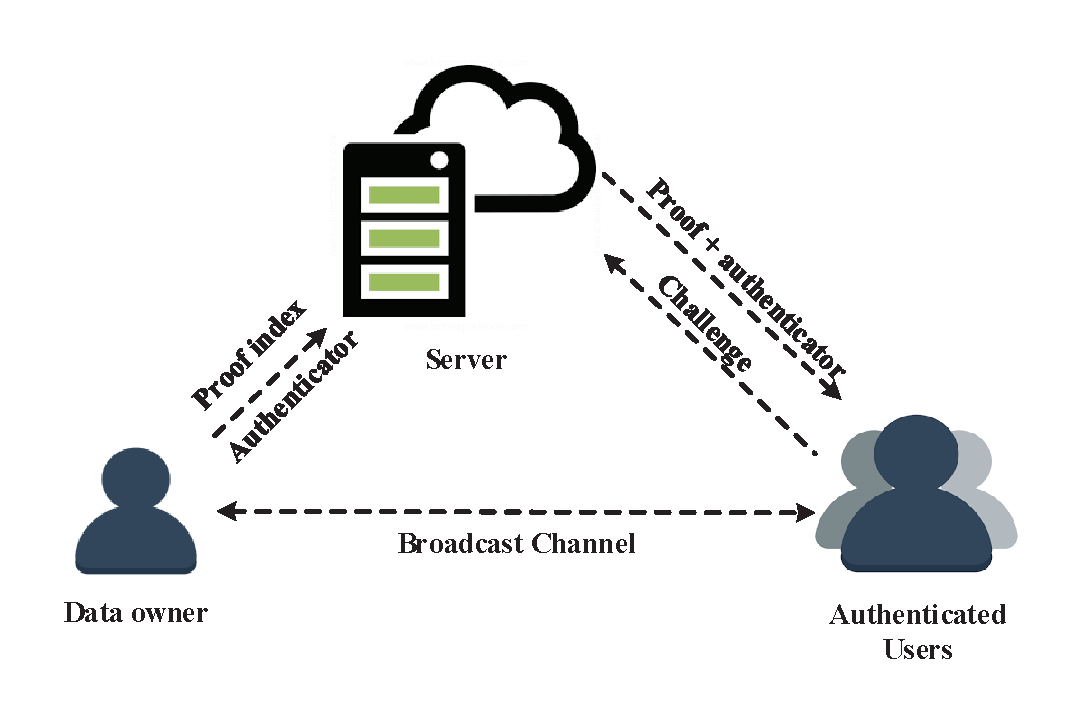
\includegraphics[width=2.5 in]{model}
\DeclareGraphicsExtensions.
\caption{System architecture of \name on the three-party model.}
\label{fig:model}
\end{figure}

In this section, we present an overview of our \name scheme. The major notations used in this paper are shown in Table~\ref{tab:notations}.

\begin{table}[h]
  \begin{center}
  \caption{Notations}
  \label{tab:notations}
  %\begin{threeparttable}
  \begin{tabular}{|c|c|}
    \hline
    Notation      &Meaning  \\
    \hline
    \hline
    $\mathcal{W}$ & keyword set \\
    \hline
    $|W|$         & \blue{size of the keyword set}   \\
    \hline
    $w_i$         & keyword, where $i \in \{1, \cdots, |W|\}$\\
    \hline
    $\mathcal{D}$ & plaintext of the document set \\
    \hline
    $D_{w_i}$     & plaintext of a document set containing $w_i$\\
    \hline
    $\mathcal{C}$ & ciphertext of the document set \\
    \hline
    $C_{w_i}$     & ciphertext of a document set containing $w_i$ \\
    \hline
    $f$           & plaintext of a document  \\
    \hline
    $c$           & ciphertext of a document \\
    \hline
    $W_f$         & keyword set of document $f$\\
    \hline
    $\tau$        & the search token (challenge)\\
    \hline
    $\lambda$     & the proof index. \\
    \hline
    $\pi$         & the authenticator.\\
    \hline
  \end{tabular}\\
  \end{center}
\end{table}


\subsection{System architechture}
Fig.~\ref{fig:model} illustrates the system architecture of \name. It consists of three parties: \blue{{\em data owners}, who provide the encrypted proof index corresponding to their data and authenticators to cloud services}; the {\em untrusted server}, which provides storage and search services; \blue{a set of {\em authenticated users}, who challenge the cloud services for verification of search results retrieved from the SSE scheme.}



\subsection{System model}
We aim to develop a verifiable SSE scheme, i.e., \name, that allows the index used for search result verification to be separated from the one used for the SSE operations. Therefore, \name is decoupled from the existing SSE schemes. \blue{In particular, data owner will builds an encrypted index based on the Merkle Patricia Tree (MPT) and upload it to cloud services, which enables data users to verify the integrity of search results. Meanwhile, data owner will also upload a timestamp-chain based on the root of MPT to ensure data freshness across multiple users.}
\name is defined as follows.

\begin{definition}[\textbf{\name Scheme}]\label{def:name}
  {\itshape
      In a \name scheme, there are three parties, i.e., data owners, authenticated users and an untrusted server.  A data owner provides a proof index and an authenticator to the untrusted server such that it allows the server to provide a proof of the search result and authenticators for the authenticated users to ensure the integrity and freshness of the SSE search results. A \name scheme is a collection of seven polynomial-time algorithms, where
      \begin{itemize}
        \item \red{$KGen(1^k) \rightarrow \{K_1,K_2,K_3, (ssk, spk)\}$: is a probabilistic algorithm run by the data owner. It takes as input a security parameter, and outputs the secret keys $K_1,K_2,K_3$ and a random signing keypair $(ssk, spk)$.}
        \item \red{$Init(K_1,K_2,K_3, ssk, \mathcal{D}) \rightarrow \{\lambda,\pi\}$: is an algorithms run by the data owner which takes as input the symmetric keys $K_1,K_2,K_3$, the signing secret key $ssk$}, and the document set $\mathcal{D}$, and outputs the proof index $\lambda$ and the anthenticator $\pi$. The data owner stores the proof $\lambda$ locally and meanwhile sends $\lambda$ and $\pi$ to the server.
        \item \red{$PreUpdate(K_1,K_2,K_3, ssk, f) \rightarrow \{\tau_u, \pi\}$: is an algorithm run by the data owner. It takes as input the symmetric keys $K_1,K_2,K_3$, the signing secret key $ssk$}, and a file $f$ to be updated, and outputs the update tokens $\tau_u$ and the authenticator $\pi$. The data owner sends $\tau_u$ and $\pi$ to the server.
        \item $Update(\lambda, \tau_u) \rightarrow \{\lambda'\}$: is an algorithm run by the server. It takes as input the proof index $\lambda$ and the update tokens $\tau_u$, and outputs the new proof index $\lambda'$;
        \item $Challenge(K_1, w) \rightarrow \{\tau_{w}\}$: is a deterministic algorithm run by the user. It takes as input a symmetric key $K_1$ and a specific keyword $w$, and outputs a challenge $\tau_{w}$ corresponding to $w$. The user sends the challenge $\tau_{w}$ to the server.
        \item \blue{$Prove(\lambda, \tau_{w}, t_q) \rightarrow \{\rho,\pi^t_q, \pi_c\}$: is an algorithm run by the server. It takes as input the proof index $\lambda$, the challenge $\tau_{w}$, and the query time $t_q$, it outputs the proof $\rho$ and authenticators $\pi^t_q$,$\pi_c$. The server sends $\rho$ and authenticators $\pi^t_q$,$\pi_c$ to the requested user.}
        \item \red{$Verify(K_1,K_2,K_3, spk, C_w, \rho, \pi^t_q, \pi_c, \tau_{w}) \rightarrow \{b\}$: is an algorithm run by the data user which takes as input symmetric keys $K_1,K_2,K_3$, the public key $spk$, the SSE search result $C_w$, the proof $\rho$, authenticators $\pi^t_q, \pi_c$ and the challenge token $\tau_{w}$, it outputs a bit $b$ represent an $accept$ or $reject$ result. This algorithm consists of two sub-algorithms,  the Check algorithm and the Generate algorithm, which can be written as $Check(K_3, spk, \pi^t_q, \pi_c) \rightarrow \{b\}$ and $Generate(K_1,K_2,K_3,C_w,\rho,\tau_{w},\pi^t_q) \rightarrow \{b\}$.}
        %\item \blue{$Verify(K_1,K_2,K_3, C_w, \rho, \pi^t_q, \pi_c, \tau_{w}) \rightarrow \{b\}$: is an algorithm run by the data user which consists of two sub-algorithms. One is the Check algorithm $Check(K_3, \pi^t_q, \pi_c) \rightarrow \{b\}$, which takes as input the tuples $<K_3, \pi^t_q, \pi_c>$, and outputs a bit $b$. The other is the Generate algorithm $Generate(K_1,K_2,K_3,C_w,\rho,\tau_{w},\pi^t_q) \rightarrow \{b\}$, which takes as input the the symmetric keys $K_1,K_2,K_3$, the SSE search result $C_w$, the proof $\rho$, the challenge token $\tau_{w}$ and the authenticator $\pi^t_q$, and it outputs a bit $b$. Finally, the Verify algorithm outputs a bit $b$ represent an $accept$ or $reject$ result.}
      \end{itemize}
      }
\end{definition}

\section{\name Construction}
\red{In this section, we present our \name construction, by starting with algorithms to build and update our proof index, and then detailed algorithms of our verification mechanism.}
%Then we use a highlevel {\it Verify} algorithm to introduce the flow of our algorithms in the following part.....organize}
%In particular, the algorithms ensure that \name can defend against the data integrity attacks and the replay attacks.}

\subsection{Building Proof Index}
%We now introduce how to build and update our proof index based on the MPT.
%\noindent\textbf{Initialization:} In the very beginning,
Algorithm~\ref{alg:Init} shows the pseudo-code of building the proof index and the authenticator (i.e., the {\it Init} algorithm defined in Definition~\ref{def:name}).
%\blue{Note that this algorithm only contains how to build the proof index, i.e., $Init(K_1,K_2, \mathcal{D}) \rightarrow \{\lambda\}$. The generation of the authenticator $\pi$ by using symmetric key $K_3$ will be described later.}
It builds a proof index with MPT structure based on the document set $\mathcal{D}$, and the inverted index $\Delta$ computed from $\mathcal{D}$, where an inverted index refers to the index \red{that} indicates the documents containing a specific keyword.
%in the SSE initialization process.
For every keyword $w_i$ in the inverted list $\Delta$, we compute the key-value pairs which will be stored in our proof index, i.e., the MPT, where the key is the token of the distinct keyword $w_i$ and the value is the incremental hash of all the documents which contain the keyword. \blue{Note that, the \red{key stores} on the path of the tree and the value stores on the corresponding leaf node.}%In later subsections, we will use the root of the MPT to verify search results.
%which will play an important role in preventing the data integrity attack,
\begin{algorithm}[t]
  \caption{$Init$}
  \label{alg:Init}
  \begin{algorithmic}[1]
    \REQUIRE ~~\\{$K_1,K_2,K_3$: the symmetric keys; \blue{$ssk$: the secret key for signing;} $\mathcal{D}$: the document set;  $F, G: \{0, 1\}^k \times \{0, 1\}^* \rightarrow \{0, 1\}^*$ the pseudo-random functions; $IH: \{0, 1\}^* \rightarrow \{0, 1\}^k$ the incremental hash functions; $H: \{0, 1\}^* \rightarrow \{0, 1\}^k$ the hash function.}
    \ENSURE ~~\\{$\lambda$: the proof index established using the MPT;
                 $\pi$: the authenticator}
              \FOR {each $w_i \in \Delta$, where $\Delta$ is the inverted index which consists of $<w_i, D_{w_i}>$ pairs}
                \STATE{$\tau_{w_i} = F_{K_1}(w_i)$}
                \STATE{$V_{w_i} = \sum_{f_i \in D_{w_i}}IH (G_{K_2} (f_i))$}
                \STATE{$\lambda = \lambda.Insert (\tau_{w_i},V_{w_i})$}
              \ENDFOR
              \STATE{\blue{Generate authenticator $\pi$ as Equation (1) with symmetric key $K_3$ and secret key $ssk$.}\footnote{\blue{The detailed explanation on the authenticator $\pi$ will be described in Section~5.3.}}}
              \RETURN $\{\lambda,\pi\}$
  \end{algorithmic}
\end{algorithm}


The {\it Update} algorithm (see Definition~\ref{def:name}) updates the proof index on the server \red{and} supports three operations, i.e., the $add$, $delete$ and $edit$ operations. Here, the $edit$ operation is equivalent to adding a new file after deleting an old file. We briefly describe the algorithm here.  First, for $add$ operations, update tokens $\tau_u$ is split into the $\{\tau_{w_i}, G_{K_2} (f)\}$ pairs, where $\tau_{w_i}$ is the token of a specific keyword extracted from the file $f$ and $G_{K_2} (f)$ is a pseudo-random string of $f$. We locate the corresponding leaf nodes based on its tokens and add the value $IH (G_{K_2} (f))$ to the existing node value. A new leaf node will be created if a token does not have a corresponding leaf node. The $delete$ operation is similar to the $add$ operation. We locate the leaf node and subtract $IH (G_{K_2} (f))$ from the value of the leaf node. Note that the {\it PreUpdate} algorithm performed by the data owner provides the tokens for the {\it Update} algorithm conducted on the server.
%The {\it PreUpdate} algorithm is similar to the {\it Update} algorithm except that the data owner can see the plaintext of its data while the server can only see the ciphertext. Here, we do not duplicate the algorithms here.

\subsection{Verifying Search Results}
\begin{algorithm}[t]
  \caption{Verify}
  \label{alg:verification}
  \begin{algorithmic}[1]
    \REQUIRE {$K_1,K_2,K_3$: symmetric keys; \blue{$spk$: the public key for verifying signature;} $C_{w}$: the search results; $\rho$: the proof of the search results; $\tau_{w}$: the challenge made by the user; $\pi^t_q$: the authenticator received in the query time $t$; $\pi_c$:  the authenticator received in the checkpoint;}
    \ENSURE {$b \in \{0,1\}$, if $b = 1$, accept; otherwise, reject.}
          \STATE {$b \leftarrow Check (K_3,\blue{spk}, \pi^t_q, \pi_c)$}
          %\IF{$b_1=1$}K_1,K_2,K_3,C_w,\rho,\tau_{w},\pi^t_q
          \RETURN {$b \leftarrow b\quad  \&\&\quad Generate(K_1,K_2,K_3,C_w,\rho,\tau_{w},\pi^t_q)$}

          %\ELSE
          %  \RETURN {$reject$}
          %\ENDIF
  \end{algorithmic}
\end{algorithm}
Algorithm~\ref{alg:verification} shows the search result verification algorithm performed by data users (i.e., {\it Verify} algorithm shown in Definition~\ref{def:name}). Firstly, it checks the correctness of the authenticator by the {\it Check} algorithm.
% that implements a timestamp-chain based mechanism.
Here, an authenticator is used to ensure the freshness of the root. %If verification is not under the replay attacks,
If the authenticator is not replayed by the server, which means the root is fresh, then we use the {\it Generate} algorithm to verify search results by leveraging the root hash value extracted from the authenticator and the proof retrieved from the server. Finally, according to the results of {\it Check} and {\it Generate}, the algorithm can determine the freshness and integrity of the search results. In the later subsections, we will elaborate the {\it Check} and {\it Generate} algorithms.

%the tree root $rt$ according to the proof $\rho$ and $D_{w}$ that is the search result of SSE such that we can compare $rt$ with the root decrypted from the authenticator $\pi^t_q$ that is received at the query time $t$. The rebuild procedure prevents the data users from the data integrity attacks. According to the check and rebuild results, the algorithm decides if the users receive correct search results. In the later subsections, we will elaborate the {\it Check} and {\it Rebuild} algorithms.}



\subsection{Verifying Authenticators}
%{\bf The replay-proof mechanism in \name (ensures replay-proof authenticators ??)used in
In order to prevent cloud services from replaying previous authenticators and ensure the freshness of the root, we maintain a timestamp-chain for authenticators\red{, such that} users can trace authenticators in the chain and identify if the root is fresh. %, which is important to ensure the correctness of search verification.
Here, the timestamp-chain scheme is different from the timestamp mechanism used in SSE~\cite{stefanov2014practical}. Their schemes can only prevent servers from constructing data freshness attacks under the two-party model when the user holds the update information. Unfortunately, it may not be able to detect data freshness attack \red{in our concerned three-party model}. We show the details of our scheme below.%}
%which will be explain in detail in the following part. \name allows users to trace back the timestamp chain and verify if a search result is replayed.}
%, we cannot directly compare timestamps in authenticators.  the mechanism can correctly verify if
%To prevent such attacks,

  \begin{figure}[htb]
    \centering
    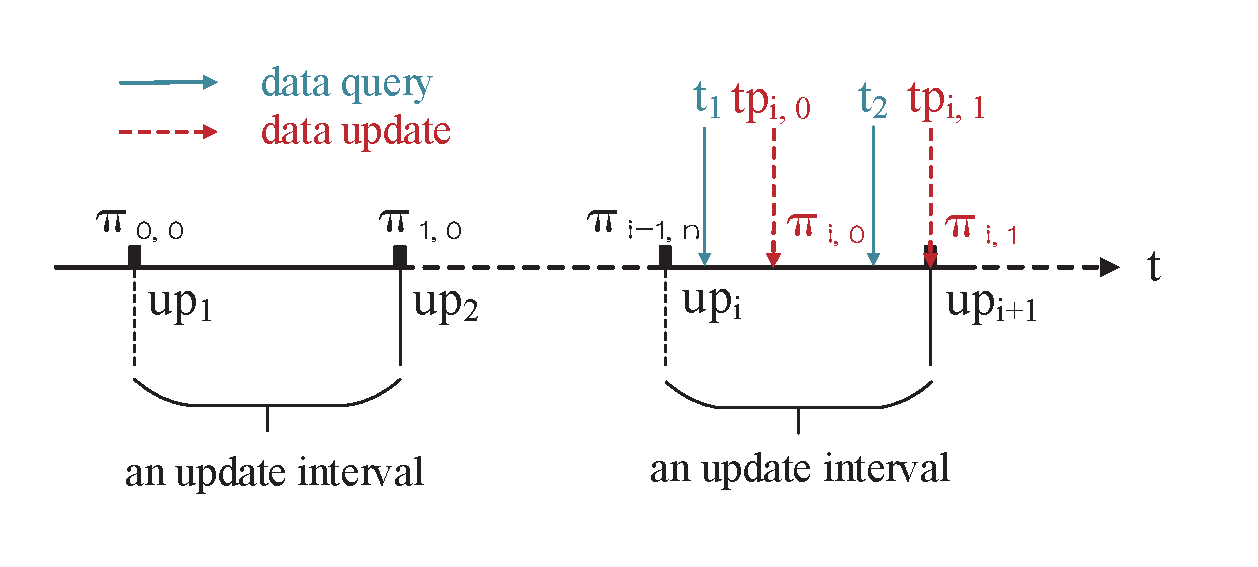
\includegraphics[width=3.5 in]{timestamp}
    \DeclareGraphicsExtensions.
    \caption{An illustration of the timestamp-chain mechanism}
    \label{fig:timestamp}
  \end{figure}

Firstly, we will show how the data owner creates the authenticator by leveraging the timestamp-chain. In the very beginning, a data owner sets an interval for authenticator update\footnote{In the performance evaluation section, i.e., Section~\ref{sec:experiments}, we will show the relationship between the update interval and the delays of detecting data freshness attacks.}, and then the fixed update time points are set to be $\{up_1, up_2, \cdots, up_i, \cdots, up_m\}$ (see Fig.~\ref{fig:timestamp}). %{\bf Here, we assume that the clock of the data owner, the data users and the cloud server is synchronized via Netword Time Protocol (NTP)~\cite{mills1991internet, mills2010network}. Some researches~\cite{kopetz1987clock, elson2002fine, zhou2007accurate} shows that the current clock synchronization accuracy can reach a few milliseconds or even tens of microseconds.}% and the network latency of them is almost the same.%The time slot between the two update points is called the update interval.
Here, we use Network Time Protocol (NTP)~\cite{mills1991internet, mills2010network} run on cloud servers
to synchronize the clocks among the data owners and the data users
during their interactions with the servers. The clock synchronization
accuracy can reach a few milliseconds or even tens of microseconds~\cite{kopetz1987clock, elson2002fine, zhou2007accurate}, and thus the accuracy is enough for verification in
GSSE. Note that, a malicious server can possibly fake a clock,
%However, it cannot fake the timestamp chain, since its goal is to allow users to successfully verify search results. a fake timestamp will olead to a fail result.
%A malicious server can indeed fake clocks,
but it cannot fake the timestamp-chain. If the server faked the clock, the timestamp will not allow a server to bypass the verification performed by users.
The authenticator is uploaded to the server periodically at the update time point when there is no data update in an update interval. \red{Otherwise}, the data owner will additionally upload the authenticators along with the updating data.
% If the proof index is not updated during an update interval, the data owner only needs to update the timestamp at the next update time point. If the dataset of the data owner is modified within an update interval, which means the proof index has been updated, then the data owner will calculate a new authenticator by using the latest root and the current timestamp and then upload it to the cloud additionally.
\begin{algorithm}[t]
  \caption{Check}
  %\setcounter{algorithm}{2.1}
  \label{alg:check}
  \begin{algorithmic}[1]
    \REQUIRE {$K_3$: the symmetric key; $spk$: the public key for verifying signature; $\pi^t_q$: the authenticator received in the query time $t$; $\pi_c$: the authenticator received in the checkpoint.}
    \ENSURE {$b \in \{0,1\}$, if $b=1$, the {\it Check} algorithm succeeds, otherwise, it fails.}
              \STATE{\blue{let $\pi^t_q = \{\alpha^t_q, Sig^t_q\}$ and $\pi_c = \{\alpha_c, Sig_c\}$}}
              \IF{\blue{$\alpha^t_q \neq (Sig^t_q)_{spk}$ $\vert \vert$ $\alpha_c \neq (Sig_c)_{spk}$}}
                \RETURN{$b = 0$}
              \ENDIF
              \STATE {$(rt^t_q, tp^t_q, \alpha) \leftarrow Dec_{K_3}(\alpha^t_q)$}
              \IF{$tp^t_q$ is not before the previous update time point}
                \STATE {let $\alpha_k = \alpha_c$}
                \FOR {$\alpha_k \neq \emptyset$}
                    \STATE {$(rt_k, tp_k, \alpha_{k-1}) \leftarrow Dec_{K_3}(\alpha_k)$}
                    \IF {$tp_k < t$}
                      \BREAK
                    \ENDIF
                    \STATE {let $\alpha_k = \alpha_{k-1}$}
                \ENDFOR
                \IF {$\alpha_k = \alpha^t_q ||\alpha_k = \emptyset$}
                  \RETURN {$b = 1$}
                \ELSE
                  \RETURN {$b = 0$}
                \ENDIF
              \ELSE
                \RETURN {$b = 0$}
              \ENDIF
  \end{algorithmic}
\end{algorithm}

Intuitively, in order to prevent the authenticator from being replayed, we can simply set the authenticator $\pi$ as a concatenation of timestamp $tp$ and the root of the MPT, i.e., the proof index, \blue{encrypt it by using a symmetric key $K_3$\red{, and then} sign it with the secret key $ssk$.} \red{If the} proof index is not updated during an update interval, the data owner only needs to update the timestamp at next update time point. If the document set of the data owner is modified within an update interval, which means the root of the proof index has been updated, then the data owner will calculate a new authenticator by using the latest root and the current timestamp and upload it to cloud services \red{again}. %{\bf In this setting, the server cannot infer relationship between authenticators during two different update intervals.??}
In this setting, when a data user generates a challenge, the server should send the latest authenticator to the data user. The data user can recover the root and the timestamp by decrypting the authenticator. If the timestamp is beyond the valid time, i.e., before the latest update time point, then the server is considered as malicious. This mechanism ensures that the server cannot mount a data freshness attack by using the data before the latest update time point.

However, cloud services may still be able to replay the authenticator between the latest update time point and the current query time. Specifically, if there is one or more data updates happened after the latest update time point, then the server can cheat the data user by sending any authenticator uploaded after the latest update time point and then mounts a data freshness attack within the latest update interval.
Therefore, we develop a timestamp-chain mechanism to detect those cheating behaviors. We modify the structure of the authenticator by \red{chaining} the value of the previous authenticator into the newly generated authenticator according to Equation (1). Note that, it will generate a new timestamp-chain of a new update interval, \red{while} the timestamp-chain ends at the beginning of the next update interval. In other words, the authenticators in each update interval are chained \red{together}, e.g., $\pi_{i, 0}, \pi_{i, 1}$ (see Fig.~\ref{fig:timestamp}), but the authenticators are irrelevant in the two different update intervals. Here, the last authenticator in each update interval is uploaded at the next update time point. In this setting, the server needs to provide an authenticator at the query time and meanwhile an authenticator at the checkpoint, where the checkpoint is referred as the next update time point closest to the user's query time $t$, e.g., $up_{i+1}$ is the checkpoint in the update interval $(up_i,up_{i+1}]$.



%In this case, the checkpoint is $up_{i+1}$.
%Therefore, the server cannot infer relationship between authenticators during two different update intervals.
%the server can cheat the maximum spoofing time of the server does not exceed the time of an update interval by using our chained-timestamp mechanism described below.

%  \begin{equation}
%    \left\{
%    \begin{array}{ll} % \begin{eqnarray}好像也可以。
%      \pi_0 = Enc_K\{rt_0||tp_0||0\cdots0\} & tp_0 = up_0\\
%      \pi_1 = Enc_K\{rt_0||tp_1||0\cdots0\} & tp_1 = up_1\\
%      \cdots & \\
%      \pi_n = Enc_K\{rt_j||tp_n||\pi_{n-1}\} & tp_n = up_i\\
%      \pi_{n+1} = Enc_K\{rt_{j+1}||tp_{n+1}||0\cdots0\} & \\
%      \pi_{n+2} = Enc_K\{rt_{j+2}||tp_{n+2}||\pi_{n+1}\} & \\
%      \pi_{n+3} = Enc_K\{rt_{j+2}||tp_{n+3}||\pi_{n+2}\} & tp_{n+3}=up_{i+1}\\
%      \cdots & \\
%    \end{array}
%    \right.
%  \end{equation}

\begin{equation}
    \left\{
    \begin{array}{ll} % \begin{eqnarray}好像也可以。
      \pi_{i, 0} = (\alpha_{i, 0}, \mathsf{Sig}_{ssk}(\alpha_{i, 0})),~~~~~~~~~~~up_i < tp_{i, 0} \leq up_{i+1} \\
      \alpha_{i, 0} = Enc_{K_3}(rt_{i, 0}||tp_{i, 0}) \\
      \cdots \\

     \pi_{i, j} = (\alpha_{i, j}, \mathsf{Sig}_{ssk}(\alpha_{i, j})),~~~~~~~~~~~tp_{i, j-1} < tp_{i, j} \leq up_{i+1}  \\
     \alpha_{i, j} = Enc_{K_3}(rt_{i, j}||tp_{i, j}||\alpha_{i, j-1}) \\
      \cdots  \\
     \pi_{i, n} = (\alpha_{i, n}, \mathsf{Sig}_{ssk}(\alpha_{i, n})),~~~~~~~~~~~tp_{i, n}=up_{i+1} \\
     \alpha_{i, n} = Enc_{K_3}(rt_{i, n}||tp_{i, n}||\alpha_{i, n-1})
    \end{array}
    \right.
  \end{equation}

\noindent \red{Here} $i$ represents the $i$-th update interval and $j$ represents the $j$-th authenticator in the interval.

Let us consider the following cases (shown in Fig.~\ref{fig:timestamp}) when a data user initiates a query at different time points: (i) the first case is that the query occurs at $t_1$, where $t_1 < tp_{i, 0}$, the server can only send $\pi_{i-1, n}$ to the data user; (ii) the second case is that the query occurs at $t_2$ after the data update event at $tp_{i, 0}$\red{, and} the authenticator that server sends to the user is $\pi_{i, 0}$; (iii) the last case is that the query is generated at $t_2$\red{, and} the authenticator sent by the server is $\pi_{i-1, n}$. In the last case, a data freshness attack occurs, but it will be detected at the checkpoint $up_{i+1}$. The data user will obtain the last authenticator $\pi_{i, 1}$ from the server at the checkpoint to verify whether the data obtained at the query time has been replayed or not.

Algorithm~\ref{alg:check} shows the pseudo-code of the {\it Check} algorithm that is executed by a data user and verifies whether the authenticator has been replayed. Let $\pi^t_q$ denote the authenticator received at the query time $t$ and $\pi_c$ denote the authenticator received at the checkpoint, which is used to deduce the previous authenticators during the latest update interval. \blue{First, we need to verify the signature of $\pi^t_q$ and $\pi_c$ by using the public key $spk$ of the data owner}. We check the authenticator $\pi^t_q$ received at the query time is not generated before the previous update time point \blue{by using $\alpha^t_q$ extract from $\pi^t_q$. Then, we decrypt the previous $rt_k||tp_k||\alpha_{k-1}$ concatenation by using $\alpha_k$ until it finds the first concatenation with timestamp $tp_k < t$ or $\alpha_k = \emptyset$. We compare $\alpha_k$ with $\alpha^t_q$ and $\emptyset$\red{. If} it is not equal to either of them, a data freshness attack is detected.} Otherwise, $\alpha^t_q$ is considered correct. Now we use the three cases above to explain the algorithm. \blue{In the first case, $\pi_{i, 1}$ and $\pi_{i, 0}$ are received and $\alpha_{i,1}$ and $\alpha_{i,0}$ are extracted. We can find the field of $\alpha$ in the concatenation is $\emptyset$ after decrypting $\alpha_{i, 0}$. Therefore, the {\it Check} algorithm outputs $b=1$ and the authenticator $\pi_{i-1, n}$ received in the query time is considered correct. In the second case, $\alpha_{i, 0}$ is also decrypted by $\alpha_{i, 1}$ and the timestamp of $\alpha_{i, 0}$ is less than $t_2$. We can find that $\alpha_{i, 0}$ and $\alpha^{t_2}_q$ are equal\red{. Hence} $\alpha^{t_2}_q$ is considered correct, i.e., $\pi^{t_2}_q$ is correct.} However, in the last case, we will detect a data freshness attack due to the mismatch between the correct authenticator $\pi_{i, 0}$ and the received one $\pi^{t_2}_q$, i.e., $\pi_{i-1, n}$.

\noindent \textbf{Remark.} The update interval can be controlled by the data owner according to its update frequency. Normally, if data is frequently updated, the update interval can be set to a shorter period so that the length of the authenticator will decrease and the verification delays will be shorter. However, it will incur more communication overheads.
%However, if the update is not frequent, the update interval can be set longer to reduce the bandwidth consumption introduced by the fixed update.
% incurred by the fixed update point.
In our experiments (see Section~\ref{sec:experiments}), we will show that the verification delays and the bandwidth consumption for updating authenticators are acceptable.
%as long as the update interval is reasonably set.
%We will prove through experiments that the cost of preventing the replay attack will not be large.


\subsection{Verifying Proofs} %Preventing Data Integrity Attacks}
\begin{algorithm}[t]
  \caption{Prove}
  \label{alg:Prove}
  \begin{algorithmic}[1]
    \REQUIRE {$\lambda$: the proof index maintained by server; $\tau_{w_i}$: the challenge made by an authenticated user; $t_q$: the query time of user.}
    \ENSURE {$\rho$: the proof of the SSE search result;
             $\pi^t_q,\pi_c$:the authenticators;}
              \STATE {Find the search path $\sigma =(n_0, \cdots, n_i, \cdots, n_m) \leftarrow \lambda.Search(\tau_{w_i})$, where $n_i \in \{EN, BN, LN\}$, $n_0$ is the root node.}
              \IF {$t_{w_i}$ exist}
                \FOR {$i = m-1$ to $0$}
                  \IF {$n_i = BN$}
                    \STATE {$\rho = \rho \cup C_{n_i}$ where $C_{n_i}$ includes several key-value pairs that are not on the search path and the key only which is on the search path $\sigma$}
                  \ELSIF{$n_i = EN$}
                    \STATE {$\rho = \rho \cup C_{n_i}$ where $C_{n_i}$ is the key which is on the search path $\sigma$}
                  \ELSE
                    \STATE{$\rho = \rho \cup C_{n_i}$ where $C_{n_i}$ is the key-value pair of node $n_i$}
                  \ENDIF
                \ENDFOR
              \ELSE %{$t_{w_i}$ not exits}
                \FOR {$i = m$ to $0$}
                    \STATE{Repeat steps 4-8}
                \ENDFOR
              \ENDIF
              \STATE{Find the latest authenticator $\pi^t_q$ according to the query time $t_q$ and the authenticator $\pi_c$ at the checkpoint.}
              \RETURN{$\rho,\pi^t_q,\pi_c$}
  \end{algorithmic}
\end{algorithm}

%In the following, we will focus on how to prevent the data integrity attack according to our proof index. We first present the prove algorithm executed on the server and then present the rebuild algorithm executed on the data user which is a part of the verify algorithm. Finally, we will explain our design by a toy example.

%\noindent\textbf{Prove:}
A user can start using the fresh root to verify the integrity of the search results after confirming that the user has obtained the correct authenticator at the query time.
In order to allow data users to generate the root of the proof index to verify search results, servers need to present proof which is generated by the {\it Prove} algorithm.
\blue{The {\it Prove} algorithm is performed by the server according to proof index $\lambda$ , the challenge $\tau_{w_i}$ (that is received from a user and corresponds to a specific keyword $w_i$) and the query time $t$}. Here, we consider both cases that the keyword is in the presence or is absence in the path of MPT. The server has to provide a proof if the keyword exists or a proof of absence if the keyword does not exist. The absence proof prevents the server from intentionally returning an empty result.

Algorithm~\ref{alg:Prove} shows the pseudo-code of generating proofs for verification (see {\it Prove} algorithm defined in Definition~\ref{def:name}). First, the server searches the proof index according to the submitted token and find the corresponding search path $\sigma$. We need to consider two cases here. If the token exists, the server needs to return the keys of each node in the search path from the bottom to the root, excluding the leaf node itself. Note that, for a branch node, we also need to return the key-value pairs that are not in the search path. However, if the token does not exist, the server also needs to return the keys of each node in the search path from the node where the search terminates to the root. Note that, we need to provide the value of the node where the search terminates. The former case is the normal one when the keyword exists, and the proof returned by the server allows the user to verify the integrity of the search results. In the latter case, the server needs to return the absence proof according to the algorithm since the proof enables the user to ensure the absence of the keyword. If the server does not follow the algorithm and returns an invalid proof, the users can detect the behaviors and the server will be treated as malicious.
\begin{algorithm}[t]
  \caption{Generate}
  \label{alg:generate}
  \begin{algorithmic}[1]
    \REQUIRE {$K_1,K_2,K_3$: the symmetric keys; $C_{w}$: the search result; $\rho$: the proof of the search result; $\tau_{w}$: the challenge made by the user himself; $\pi^t_q$: the root received at the query time.}
    \ENSURE {$b \in \{0,1\}$, if $b=1$, the {\it Generate} algorithm succeeds, otherwise, it fails.}
          \STATE {Compute $\{remain\_key\}$ = String.match ($\tau_{w_i}$, keys in $\rho$)}
          \IF {$C_{w} = \emptyset$ \&\& $remain\_key = \emptyset$}
              \STATE {Calculated the root $rt$ according to $\rho$ from the bottom to root.}
          \ELSIF {$C_{w} \neq \emptyset$ \&\& $remain\_key \neq \emptyset$}
              \STATE {Compute $\varphi = \sum_{f \in D_{w}}IH (G_{K_2} (f_i))$, where $D_w$ is the plaintext of $C_w$}
              \STATE {Compute $LN = Compute(\varphi, remain\_key)$}
              \STATE {Calculated the root $rt$ according to $LN$ and $\rho$ from the bottom to the root.}
          \ELSE
              \RETURN {$0$}
          \ENDIF
          \STATE {$(rt^t_q, tp^t_q, \pi) \leftarrow Dec_{K_3} (\alpha^t_q)$, where $alpha^t_q$ is extract from $\pi^t_q$;}
          \IF{$rt = rt^t_q$}
            \RETURN{$1$}
          \ELSE
            \RETURN{$0$}
          \ENDIF
  \end{algorithmic}
\end{algorithm}

%  \noindent\textbf{Rebuild:}
After receiving the proof from the server, the data user needs to generate the tree root, which is performed by the {\it Generate} algorithm (see in Definition~\ref{def:name}). The pseudo-code is shown in Algorithm~\ref{alg:generate}. It first compares the challenge $\tau_{w}$ with the keys in $\rho$. If the keys in $\rho$ is not the prefix of $\tau_{w}$, $remain\_key$ is set to $\emptyset$. Otherwise, $remain\_key$ stores the remaining bits of $\tau_{w}$. If both the search result and $remain\_key$ are $\emptyset$, we can generate the tree root $rt$ according to the proof $\rho$. If both the search result and the $remain\_key$ is not $\emptyset$, we need to calculate the corresponding leaf node according to the search result and the $remain\_key$, and then \red{generate} the tree root $rt$ by using the calculated leaf node and the proof $\rho$. \red{If it's neigher of the above two cases, the server is considered malicious, the server is considered malicious.} Finally, we compare the calculated root $rt$ with the correct one $rt^t_q$ to verify the correctness of the root $rt$. If they are not equal, it means the server has tampered with \red{either} the proof $\rho$ or the search result, \red{and thus} the verification fails.
%(see Algorithm~\ref{alg:verification}).}

%If the search result is empty, we need to confirm the absence of challenge $t_{w_i}$ by checking the $remain\_key$ and then generate the tree root according to the proof $\rho$. If the search result is not empty, we can calculate the corresponding leaf node by the search result and the $remain\_key$. Finally, it generates the tree root by using both the calculated leaf node and the proof $\rho$. The data user can detect the data integrity attacks by comparing the calculated root with the correct one.
\subsection{\red{An Illustrative Example}}

  \begin{figure*}[t]
  \centering
  \includegraphics[width=7 in]{mpt}
  \DeclareGraphicsExtensions.
  \caption{An illustrative example}
  \label{fig:mpt}
  \end{figure*}

We use an example shown in Fig.~\ref{fig:mpt} to exemplify the algorithms operating the proof index. We assume that initially there are four documents, i.e., $\{f_1, f_2, f_3, f_4\}$, which consist of four different keywords $\{w_1, w_2, w_3, w_4\}$ presented in the inverted list (see the left part of Fig.~\ref{fig:mpt}). Keyword $w_1$ is contained in all documents\red{. Keyword} $w_2$ is only contained in document $f_2$\red{. keywords} $w_3$ and $w_4$ are contained in $\{f_1, f_2, f_3\}$ and $\{f_1, f_2, f_4\}$ \red{respectively}. The corresponding tokens and values of keywords are also given in the inverted list. Initially, we build the proof index by inserting the key-value pairs into MPT. For an update operation, e.g., adding a new file $f_5$ that \red{contains} $w_2$ and $w_5$, the update tokens are split into [`a5432', $IH(G_{K_2} (f_5))$] and [`a5fab', $IH(G_{K_2} (f_5))$]. For the token `a5432' that already exists, we only need to add $IH(G_{K_2} (f_5))$ to the original node value $IH(G_{K_2} (f_2))$. For the new token `a5fab', we need to create a new node and assign the value $IH(G_{K_2} (f_5))$ to it. Note that any change to the node will trigger a change of the hash value in the root node.

Suppose a user wants to search the keyword $w_2$ and submits the corresponding token `a5432' which already \red{exists} in the proof index. The search path of this token is \{BN1,EN1,BN2,LN3\}, and the proof $\rho$ produced by the {\it Prove} algorithm should be [$C_{n_2}, C_{n_1}, C_{n_0}$] (see Fig.~\ref{fig:mpt}). After receiving the proof $\rho$ from the server, the data user runs the $Generate$ algorithm to check the integrity of the search result. For simplicity, here, we assume that all root hash values in this example are verified by the {\it Check} algorithm. First, the $remain\_key$ `32' is calculated by string matching. Specifically, `a',`5',`4' can be found in $C_{n_0}, C_{n_1}, C_{n_2}$, so the $remain\_key$ is `32'. Then the first shaded area in $\rho$ is calculated based on the $remain\_key$ and the search results of the SSE scheme. Namely, for keyword $w_2$, the search result of the SSE scheme should be file $f_2$ and $f_5$. The user needs to recompute the value of LN3 by binding the $remain\_key$ `32' with the sum of $IH(G_{K_2} (f_2))$ and $IG(G_{K_2} (f_5))$. If the server does not cheat, the value should be equal to the value of LN3. After retrieving the value of the first shaded part, we can generate the root hash according to the proof $\rho$. {If there is an attack, e.g., the server only returns the file $f_2$ that is the result before the update of file $f_5$, the rebuilt root hash value will also be the root hash before the update\red{. Then} the {\it Generate} algorithm will fail.}

\red{Now suppose} the user submits a token that does not exist in the proof index, e.g., token `a5433'. The search path in the tree terminates in the leaf node LN3, which is the same to the search path of `a5432'. The proof $\rho$ returned by the server should be [$C_{n_3}, C_{n_2}, C_{n_1}, C_{n_0}$] (see Fig.~\ref{fig:mpt}). %The $remain\_key$ `33' is firstly calculated. Specifically,
The user first confirms that the first bit `a' of the token is present in $C_{n_0}$, and then \red{confirms} that `5' and `4' are in $C_{n_1}$ and $C_{n_2}$, respectively. It is obvious that `33' does not exist in $C_{n_3}$, \red{thus $remain\_key$ is set to $\emptyset$}, which indicates the keyword does not exist. %Follow the {\it Rebuild} algorithm,
Then, the user generates the root hash based on the proof by using {\it Generate} algorithm and compares it with the root extracted from the authnticators. Note that, any small changes in the proof $\rho$ will affect the value of the final root hash. Therefore, users can easily detect if the server tampered with the proof $\rho$, and then ensure the integrity of the search results.


%\noindent \textbf{Remark.} We present a fully dynamic proof index, propose a Prove algorithm and a Rebuild algorithm against the data integrity attacks. From the details of our algorithms, we can see that the Merkle Tree scheme \cite{kamara2011cs2} can not prevent the server from ignoring all the files and is incomplete for preventing the data integrity attack. Notice that we do not directly provide the value of the leaf node corresponding to the challenge as a proof. Instead, we give the key-value pairs of each node on the search path as our proof for the following two reasons: First, when the server claims an absence of a keyword, the key-value pairs along the search path are necessary to enable the user to verify whether the keyword exits or not; Second, the subsequent detection of the replay attack is implemented by using the tree root, so it is necessary to bind the tree root with the proof to ensure that the proof is not replayed.
%\subsection{Verification}

\section{Security Analysis}
In this section, we give a rigorous security analysis of our \name scheme.
We plan to demonstrate the security of \name on two aspects, i.e., confidentiality and verifiability. \red{Confidentiality means an adversary cannot learn any useful information about files and keywords through the proof index and update tokens used in \name}, while verifiability means that result verification will not output an accept when the search result received from cloud services is incorrect or incomplete. First, we adopt the $\mathbf{Real/Ideal}$ simulation in \cite{kamara2011cs2} to prove confidentiality of \name.

\begin{definition}[\textbf{\name confidentiality}]
  {\itshape
    Let the \name scheme be a dynamic verifiable scheme based on the searchable symmetric encryption and consider the following probabilistic experiments, where $\mathcal{A}$ is a stateful adversary, $\mathcal{S}$ is a stateful simulator, and $\mathcal{L}$ are stateful leakage algorithms:

    $\mathbf{Real}_\mathcal{A}(k)$: a challenger runs $KGen(1^k)$ to generate symmetric keys {$K_1,K_2,K_3$}. The adversary $\mathcal{A}$ chooses a document set $\mathcal{D}$ for the challenger to create a proof index $\lambda$ and an authenticator $\pi$ via $\{\lambda,\pi\} \leftarrow Init(K_1,K_2,K_3,\mathcal{D})$, and makes a polynomial number of adaptive queries $q = \{w,f\}$. For each query $q$, $\mathcal{A}$ receives from the challenger a challenge token $\tau_w$ such that $\tau_w \leftarrow Challenge(K_1,w)$, an update token and the authenticator $(\tau_u,\pi)$ such that $(\tau_u,\pi) \leftarrow PreUpdate(K_1,K_2,K_3,f)$. Finally, $\mathcal{A}$ returns a bit $b$.

    $\mathbf{Ideal}_\mathcal{A,S}(k)$: The adversary $\mathcal{A}$ chooses a document set $\mathcal{D}$. Given $\mathcal{L}(\mathcal{D})$, the simulator $\mathcal{S}$ generates and sends proof index $\tilde{\lambda}$ and the authenticator $\tilde{\pi}$ to $\mathcal{A}$. The adversary $\mathcal{A}$ makes a polynomial number of adaptive queries $q = \{w,f\}$. For each query $q$, $\mathcal{S}$ returns the appropriate token $\tau$ and the authenticator $\pi$. Finally, $\mathcal{A}$ returns a bit $b$.

    We say that SSE is $\mathcal{L}$-confidential if for all probabilistic polynomial-time  (PPT) adversaries $\mathcal{A}$, there exists a PPT simulator $\mathcal{S}$ such that $$|Pr[\mathbf{Real}_A(k) = 1] - Pr[\mathbf{Ideal}_{A,S}(k) = 1]| \leq negl(k).$$
  }
\end{definition}

Before proving the confidentiality, we formalize the view of the adversary as follows: $\mathcal{L}(\mathcal{D})$ = $(|\lambda|,|\pi|,\{\tau\}_q,\{\sigma\})$\red{. Here} $|\lambda|$ is the size of the proof index \red{indicated} by the number of leaf nodes\red{. $\pi$} is the length of the authenticator\red{. $\{\tau\}_q$} are $q$ tokens which are adaptively generated\red{. $\{\sigma\}$} are the search paths in the proof index, e.g., all the tokens correspond to the set of keywords $\mathcal{W}$. Then we have the following theorem.

\begin{theorem}
  {\itshape
    The \name scheme is $\mathcal{L}$-confidential if $F$ and $G$ are pseudo-random functions.
  }
\end{theorem}

\begin{proof}
  We show that there exist a polynomial-time simulator $\mathcal{S}$ such that for all probabilistic polynomial time (PPT) adversaries $\mathcal{A}$, the output between the real game $\mathbf{Real}_\mathcal{A}(k)$ and a simulation game $\mathbf{Ideal}_\mathcal{A,S}(k)$ is computationally indistinguishable.

  First of all, given $\mathcal{L}(\mathcal{D})$ = $(|\lambda|,|\pi|,\{\tau\}_q,\{\sigma\})$, $\mathcal{S}$ simulates the proof index $\tilde{\lambda}$ by choosing $|\lambda|$ random key-value strings and inserting into MPT. Meanwhile, $\mathcal{S}$ chooses a random  string $\tilde{\pi}$ with length $|\pi|$. Recall that each key-value pair in MPT is encrypted by the pseudo-random function $F$ and $G$\red{, and} the confidentiality of the authenticator is essentially ensured by the underlying cipher\red{. Therefore,} $\mathcal{A}$ cannot differentiate $(\tilde{\lambda},\tilde{\pi})$ from $(\lambda,\pi)$.
  Now let $\mathcal{S}$ simulates challenge tokens. For the first token $\tau_w$, if it matches one search path in $\{\sigma\}$, then $\mathcal{S}$ chooses a random path in $\tilde{\lambda}$ as the challenge token $\tilde{\tau_w}$ and returns it to $\mathcal{A}$.  Otherwise, $\mathcal{S}$ chooses a random string which is not in the search path of $\tilde{\lambda}$. Thus, $\mathcal{A}$ cannot differentiate the real token from the simulated token. For the subsequent tokens, if $w$ has appeared before, then the challenge token $\tilde{\tau_w}$ is the same to the previous one or follows the same way of simulating the first token. \red{In either case, the} challenge token $\tilde{\tau_w}$ is returned to $\mathcal{A}$ \red{accordingly}.
% who cannot differentiate tokens either.
  Similarly, when $\mathcal{A}$ simulates an update token, the update token is set to $\tilde{\tau_u} = (\tilde{\tau_{w_1}},\cdots,\tilde{\tau_{w_{|W_f|}}},\tilde{\tau_r})$ and the authenticator $\tilde{\pi}$ is set as a random string with the same length as $\pi$. For each $\tilde{\tau_{w_1}}$, $\mathcal{A}$ chooses the random string as the same way in simulating the challenge tokens.
  Since all tokens in the $\mathbf{Real}_\mathcal{A}(k)$ game was encrypted by the pseudo-random function $F$, the adversary $A$ cannot differentiate the simulated tokens from the real tokens. Therefore, we can conclude that the outputs of $\mathbf{Real}_\mathcal{A}(k)$ and $\mathbf{Ideal}_\mathcal{A,S}(k)$ are indistinguishable.
\end{proof}

 The verifiability of the \name scheme means that the scheme can verify the freshness and integrity of the search results, i.e., prevent the data freshness attack and data integrity attack defined by Definition~\ref{def:freshness} and Definition~\ref{def:integrity}. Here, we adopt a game-based security definition to prove the verifiability of \name.
\begin{definition}[\textbf{\name verifiability}]
  \itshape{
      Let the \name scheme be a dynamic verifiable scheme based on the searchable symmetric encryption and consider the following probabilistic experiments, where $\mathcal{A}$ is a stateful adversary:

      \noindent$\mathbf{Vrf}_\mathcal{A}(k)$:
      \begin{enumerate}[1.]
        \item the challenger runs $KGen(1^k)$ to generate symmetric keys {$K_1,K_2,K_3$}.
        \item the adversary $\mathcal{A}$ chooses a document set $\mathcal{D}$ for the challenger.
        \item the challenger \red{creates} a proof index $\lambda$ and an authenticator $\pi$ via $\{\lambda,\pi\} \leftarrow Init(K_1,K_2,K_3,\mathcal{D})$,
        \item given $\{\lambda,\pi\}$ and oracle access to $Challenge(K_1,w)$ and $PreUpdate(K_1,K_2,K_3,f)$, the adversary $\mathcal{A}$ outputs a keyword token $\tau_w$, a sequence of files $C'$ such that $C' \neq C_w$, the authenticators $\pi_q',\pi_c'$ and a proof $\rho'$.
        \item the challenger computes $b:=Verify(K_1,K_2,K_3,C_w,\rho,\pi_q',\pi_c',\tau_w)$.
        \item the output of the experiment is the bit b.
      \end{enumerate}
      We say that \name is verifiable if for all PPT adversaries $\mathcal{A}$, $$Pr[\mathbf{Vrf}_\mathcal{A}(k)=1] \leq negl(k).$$
  }
\end{definition}

\begin{theorem}
  {\itshape
    The \name scheme is verifiable if the hash function $H$ and the incremental hash function $IH$ are collision-resistant and $G$ is pseudo-random.
  }
\end{theorem}

\begin{proof}
Considering the situation where a search result $\tilde{D_w}$ returned by the server is different from the correct answer $D_w$ but the {\it Verify} algorithm accepts the search result $\tilde{D_w}$. In order to \red{ensure} the \name scheme is verifiable, we only need to prove verifiability of {\it Check} and {\it Generate} algorithms. First, for the {\it Check} algorithm, since the authenticator $\pi$ is encrypted by \red{the data owner, its unforgeability is guaranteed by the underlying AES ciphers and digital signature. Anyone without the secret signing key $ssk$ and symmetric key $K_3$ cannot generate the authenticator that can be authenticated by the data user.} Second, for the {\it Generate} algorithm, there are two possible scenarios to output two collision root hash\red{. The} first is that $\tilde{D_w}$ and $D_w$ induce a collision of the incremental hash function $IH$. \red{The other} is that the collision occurs in the path when computing the root hash of the proof index. However, the probability that a hash function produces a collision is less than a negligible value, so the verifiability of the {\it Generate} algorithm is guaranteed. Therefore, \red{the \name scheme is indeed} verifiable.
\end{proof}

\section{Performance Evaluation}~\label{sec:experiments}
%In this section, we present

% \blue{In this section, we present experimental results to measure the efficiency and communication overhead of our scheme.}
% and macrobenchmark experiments to demonstrate its performance in large-scale database.

\subsection{Experiment Setup}
In order to demonstrate the feasibility of \name, we \red{have implemented} it by using Crypto++ 5.6.5. The prototype is written by about 2200 lines of code. %Our implementation includes all the algorithms mentioned in section \uppercase\expandafter{\romannumeral4}.
\blue{We use 128-bit AES-CBC to encrypt the authenticators and sign it with RSA signature.} We implement two random-oracles with HMAC-SHA256 and the hash function is an implementation of SHA3-256 and the incremental hash function is MuHash.
%
Our experiments were performed by using a machine with single thread on an Intel Core i5 2.5GHz processor with 4G RAM. %All experiments w performed
We used the Enron email dataset~\cite{enron_email} in our experiments. The used part of the dataset~\cite{enron_email} is between ``allen-p" and ``kaminski-v". We extract document-keyword pairs from the dataset and construct our plaintext inverted index by using a python script. Note that the delays of extracting keywords from files are not included in our evaluation, since keyword extraction is independent with \name.
\red{We first measure the overheads of the algorithms proposed and then compare \name with a well-known SSE scheme~\cite{cash2014dynamic} to demonstrate the small extra overhead introduced by result verification.}

% Here, we measure the average results with ten runs of experiments.

%In macro-benchmark experiments, we evaluate the \name performance in large-scale database by feeding the measured delays and then we compare \name with the existing SSE scheme~\cite{cash2014dynamic}.
%Each data point in the graphs is an average of ten trials.
%The part of the Enron email dataset that we used in our experiments is between "allen-p" and "kaminski-v".
\subsection{Experimental Results}


\begin{figure*}[bhpt]
\centering
  \begin{minipage}[b]{0.33 \textwidth}
    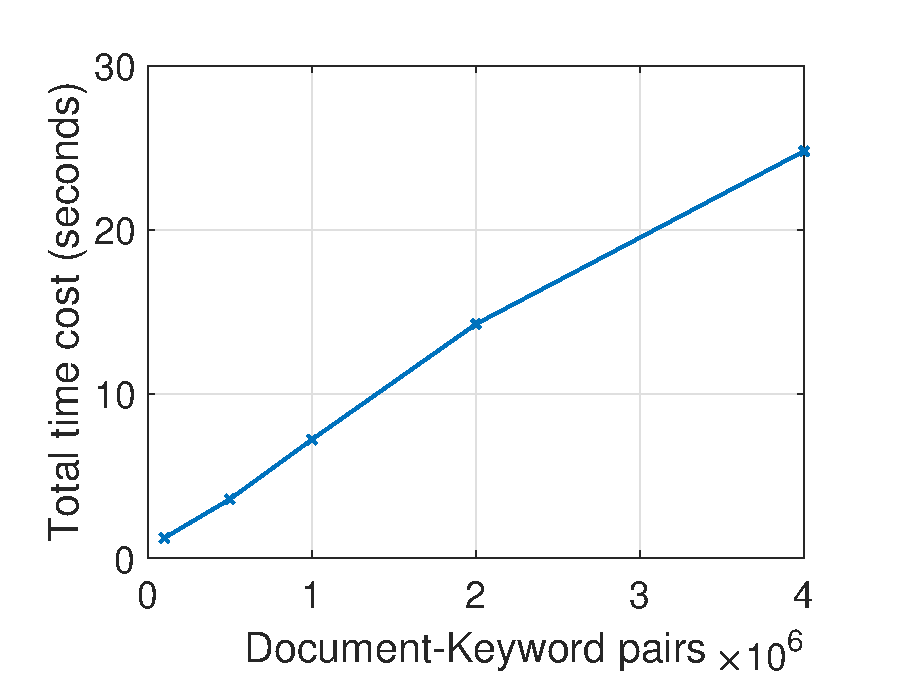
\includegraphics[width=\textwidth]{initialization}
    \caption{$Init$ delays}
    \label{fig:initialization}
  \end{minipage}
  \hspace{-0.2in}
  \begin{minipage}[b]{0.33 \textwidth}
    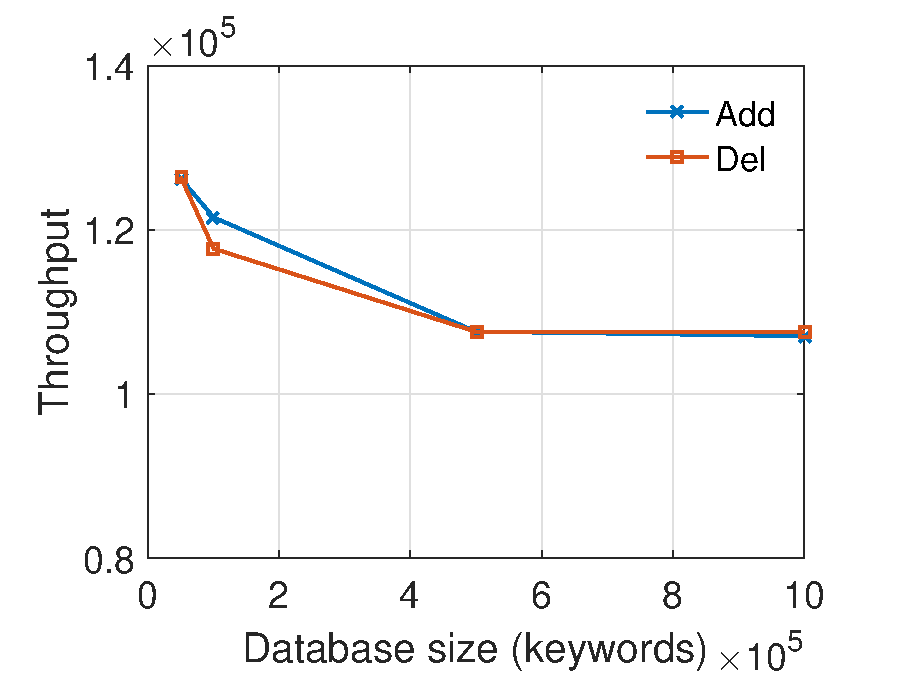
\includegraphics[width=\textwidth]{update}
    \caption{$Update$ throughput}
    \label{fig:update}
  \end{minipage}
  \hspace{-0.3in}
  \begin{minipage}[b]{0.33 \textwidth}
    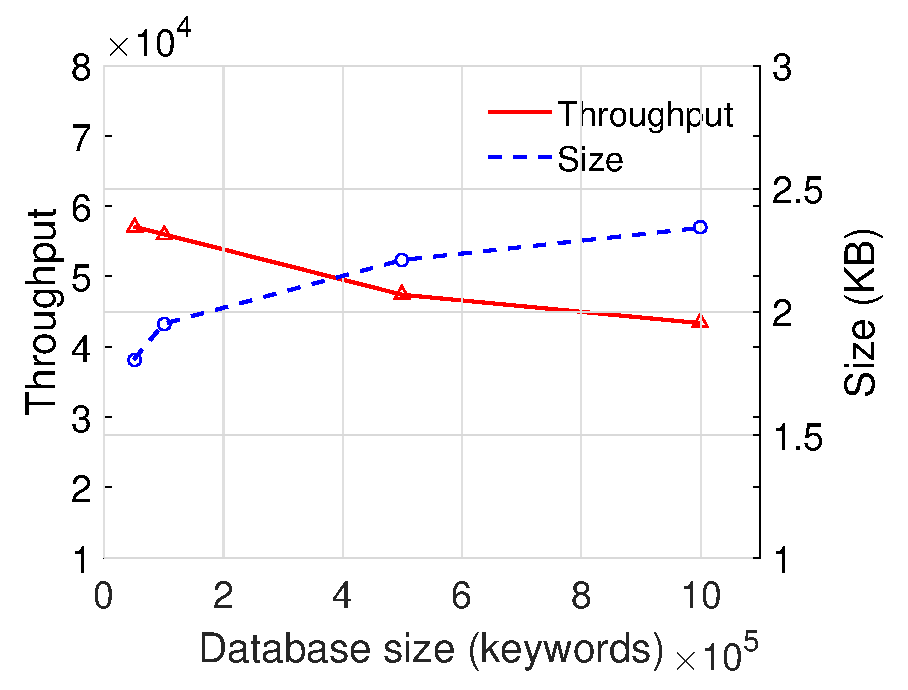
\includegraphics[width=\textwidth]{prove}
    \caption{$Prove$ cost}
    \label{fig:prove}
  \end{minipage}

  \hspace{-40.0pt}
  \par \vspace{-10.pt}
  \hspace{-36.0pt}

  \begin{minipage}[b]{0.33 \textwidth}
    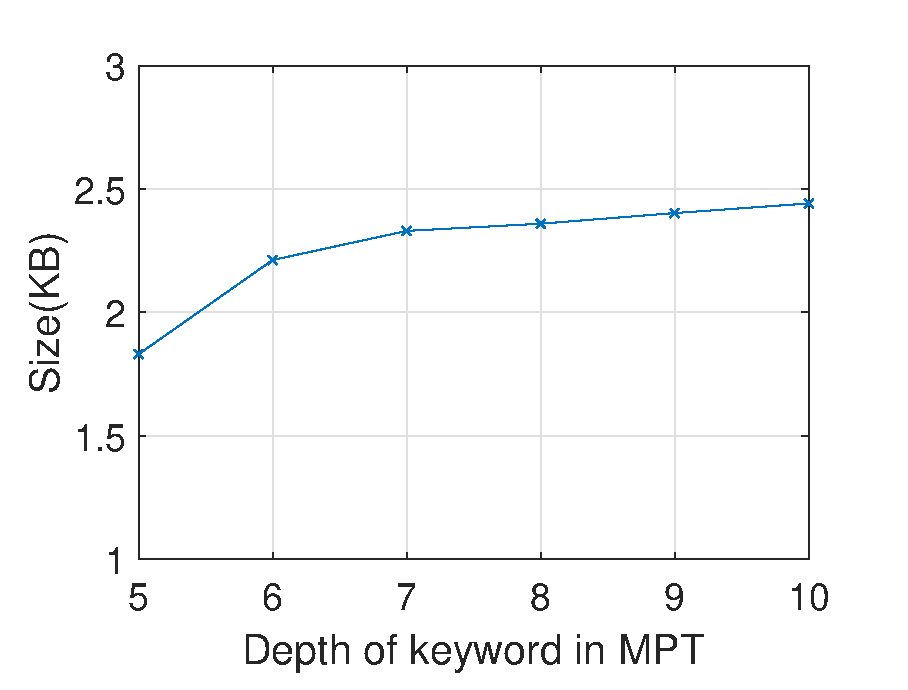
\includegraphics[width=\textwidth]{proof}
    \caption{\blue{Proof cost of MPT}}
    \label{fig:proof}
  \end{minipage}
  \hspace{-0.2in}
  \begin{minipage}[b]{0.33 \textwidth}
    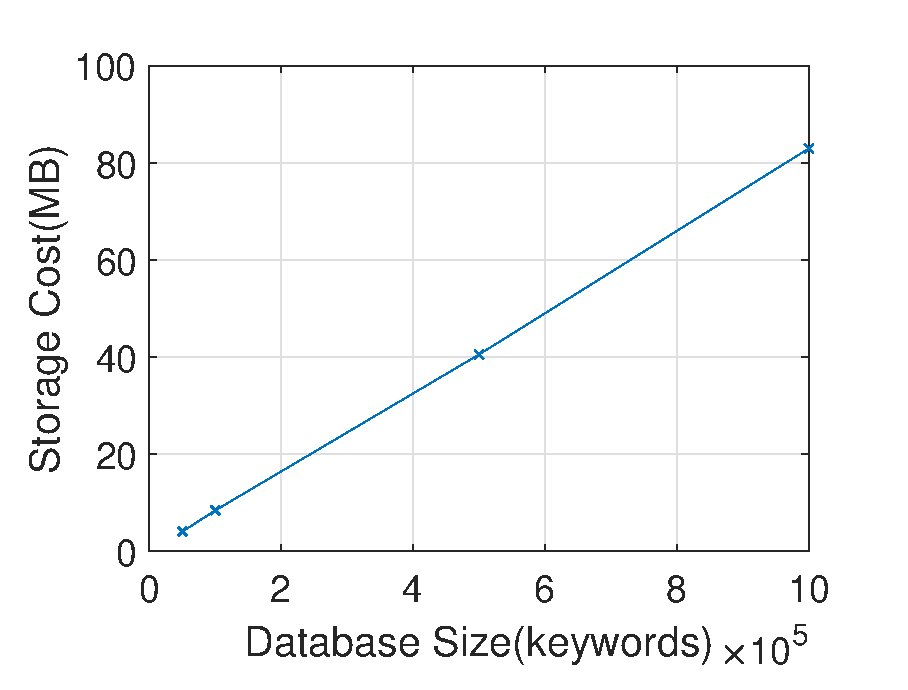
\includegraphics[width=\textwidth]{storage}
    \caption{Storage cost of MPT}
    \label{fig:storage}
  \end{minipage}
  \hspace{-0.2in}
  \begin{minipage}[b]{0.33 \textwidth}
    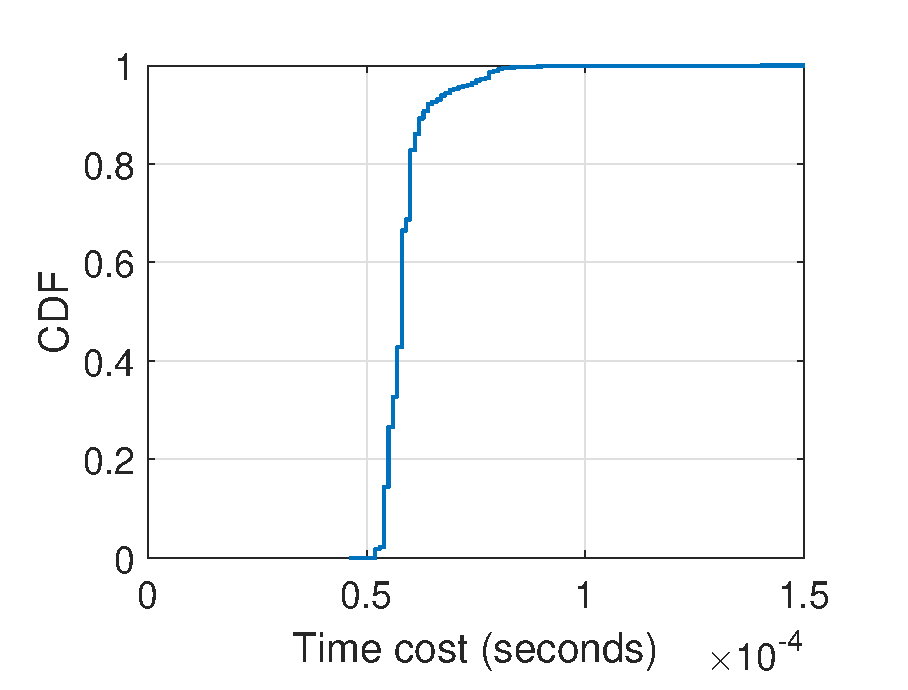
\includegraphics[width=\textwidth]{generate}
    \caption{$Generate$ performance}
    \label{fig:generate}
  \end{minipage}

  \hspace{-40.0pt}
  \par \vspace{-10.pt}
  \hspace{-36.0pt}

  \begin{minipage}[b]{0.33 \textwidth}
    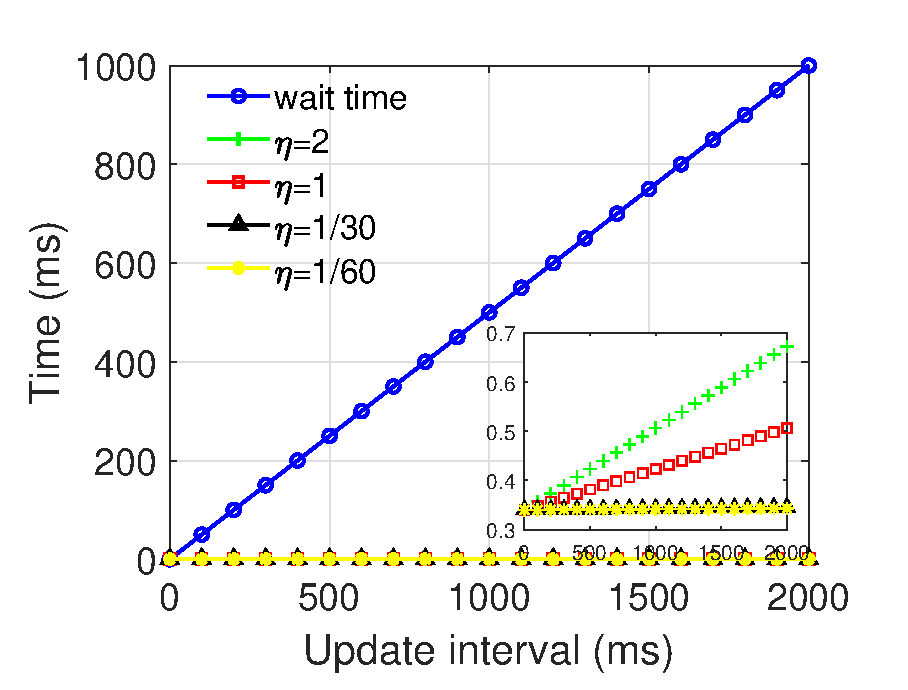
\includegraphics[width=\textwidth]{verify}
    \caption{$Verify$ latency}
    \label{fig:verify}
  \end{minipage}
  \hspace{-0.2in}
  \begin{minipage}[b]{0.33 \textwidth}
    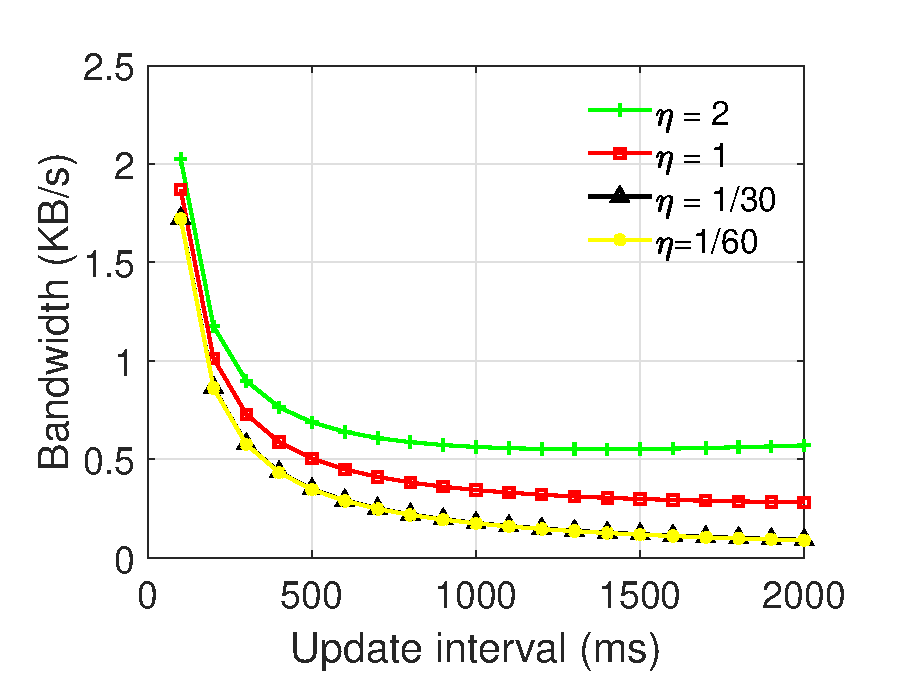
\includegraphics[width=\textwidth]{bandwidth}
    \caption{Bandwidth consumption}
    \label{fig:authenticator bandwidth}
  \end{minipage}
  \hspace{-0.2in}
  \begin{minipage}[b]{0.33 \textwidth}
    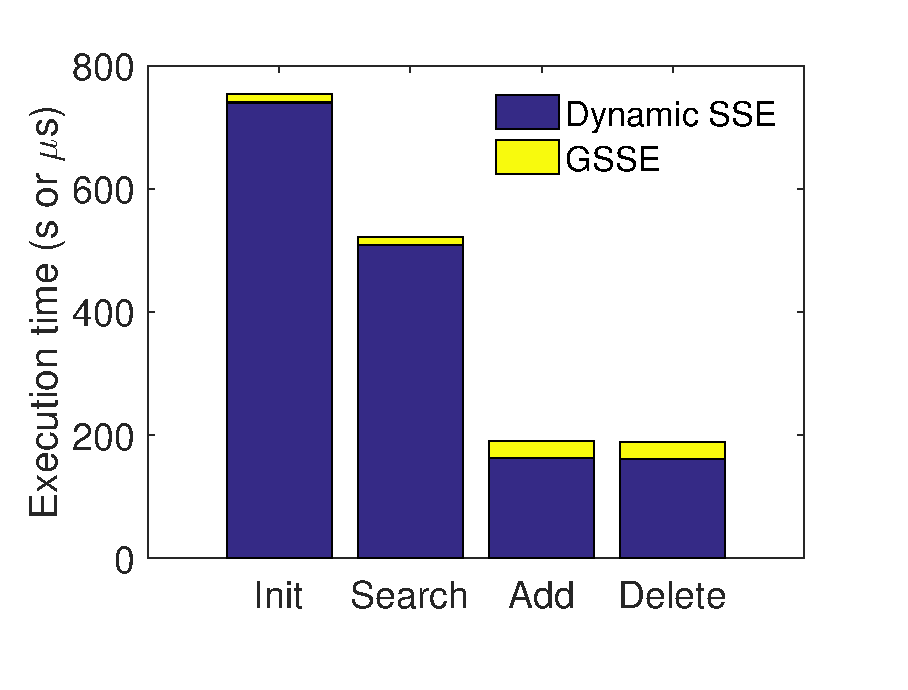
\includegraphics[width=\textwidth]{comparison}
    \caption{\blue{Comparison with SSE~\cite{cash2014dynamic}}}
    \label{fig:comparison}
  \end{minipage}
\centering
\end{figure*}


\blue{First, we measure the delays of the \emph{Init} algorithm as shown in Fig.~\ref{fig:initialization}, which include the building of the proof index and the authenticator. \red{All the delays and the subsequent measurements are the average results with ten runs of experiments.} Note that the cost of building the authenticator is negligible.}
The delays of generating the proof index are proportional to the size of the document-keyword pairs, since \name performs the same number of insertions to the number of the document-keyword pairs. Overall, the initialization consumes around 25 seconds where the documents include four million keywords, which is acceptable.
% for the initialization process.

The update delays are decided by the size of the database that is measured by the number of keywords.
%The size of MPT grows with the increase in the number of keywords.
Strictly speaking, the delays are directly related to the number of the layers in MPT. In order to show the relationship between the update delays and the database size, we use various numbers of keywords to measure the delays. Since the number of keywords varies from each file, we use throughput to measure the number of keyword-document pairs that can be updated per second (see Fig.~\ref{fig:update}). We observe that the throughput of adding and deletion operations are almost the same. The throughput decreases when the size of the database grows. They can support 110,000 updates per second with one million keywords database.
Similarly, we observe that the bandwidth overhead incurred by update token is decided by the number of keywords contained in the file. \blue{Each update token takes about 32 bytes, which is acceptable as well.}

%\subsection{Microbenchmark: {\it Prove} and {\it Rebuild}}
%We use throughput to measure our prove algorithm. Prove process is actually the process of searching and tracing back in the proof index. As a result, the performance
As shown in Fig.~\ref{fig:prove}, the server can perform about 43,000 prove operations per second even when the size of the database is one million keywords, which indicates the server can simultaneously support 43,000 concurrent queries submitted by users. \blue{Note that this experiment only measures the cost of generating the proofs, not including the \red{waiting} time for the authenticator in the checkpoint.}
%the throughput of {\it Prove} is better that the {\it Update} algorithm.
The communication overhead incurred by proof delivery is only a few kilobytes, which is decided by the number of layers in MPT, and gradually increases as the database grows (see Fig.~\ref{fig:prove} and Fig.~\ref{fig:proof}).

\blue{We measure the storage cost MPT as shown in Fig.~\ref{fig:storage}. If we use a database with 1,000,000 keywords, the storage overhead is about 82MB. Compared with the size of the original dataset itself, \red{590~MB}, the overhead is relatively small. Note that, if a data owner stores various media types of data set (e.g., images or music) with fewer keywords or attributes, the storage overhead of MPT \red{will further reduce to be practically negligible,} compared with the size of the data set itself.}

\blue{The performance of {\it Generate} algorithm performed by data users is presented in Fig.~\ref{fig:generate}.}
% and usually is not frequent operations.  %Hence, we only measure the delays of rebuilding operations. % rather than the throughput. We prove through experiments that
We observe that the \red{measured} delays of generating root are \red{all} within 0.1 milliseconds and are acceptable.

%For a 590MB database with 1,000,000 keywords, the storage cost of the MPT is only about 82MB. As the data set (aka, the Enron email) contains a large number of keywords, the storage space of MPT is relatively large. Note that, if a data user stores various media types of data set (e.g., images or music) with fewer keywords or attributes, the storage overhead of MPT is negligible compared with the size of the data set itself.


%\subsection{Macrobenchmark}
%The cost of preventing the replay attack consists of the following two parts: the computational cost of the data user for executing the verify algorithm and the communication cost of the data owner for updating the authenticator. Here we evaluate the cost of preventing the replay attacks from these two aspects.
%In this experiment, we measure the delays of verification and the communication overhead in data owners. %Here, we assume that, for a data owner, the data update frequency is constant.  %represented by $\eta$ is constant, and the update interval is represented by $\alpha$.
\blue{In Fig.~\ref{fig:verify}, we evaluate the verification delays in data users.} Note that an entire verification delay includes the delay of waiting for a checkpoint and the delay of executing the {\it Check} and the {\it Generate} algorithms. Since the execution delay of the {\it Generate} algorithm is relatively stable, \blue{\red{around} 0.1 milliseconds,} we do not plot it in Fig.~\ref{fig:verify}. Here, $\eta$ is the update frequency of the data owner\red{.} \red{We assume that the} time that a user initiates a query is uniformly distributed during an update interval, and then the user's waiting delays are also uniformly distributed. Therefore, the expected delay is half of the update interval and the verification delays are dominated by the waiting delays. \blue{The execution delay of the {\it Check} algorithm is negligible and is proportional to the update interval, which is mainly incurred by verifying the signature and decrypting authenticators.} 
\red{Kindly note that in above measurement, we do not take into account the network transmission and propagation delays, as they vary in different specific network contexts and do not reflect the essential extra cost directly introduced by our verification design. We do, however, report the communication overhead in terms of the message size, as shown in Fig.~\ref{fig:authenticator bandwidth}}. In a later experiment, we will also show that we can set an update interval so as to make a trade-off between verification delays and communication overhead.
%As we observed, the average delay for decrypting each authenticator is only about 0.12 milliseconds.
%Overall, the verification delay is around 500 milliseconds.}
%is negligible compared with the waiting delays,
%We observe that the verification delays are dominated by the waiting delays.
%delays of performing the {\it Check} algorithm. We observe that the execution delay of the {\it Check} algorithm is proportional to the number of rounds that are required to trace back in the timestamp chain. %As the worst case, the delay is  to the number of rounds of tracing back.
%If the data update frequency is constant for a specific data owner, then the execution delays will be proportional to the update interval.}
%We denote the average decryption time of an authenticator as $avg(Dec_K(\pi))$. Then the execution time of the check algorithm can be evaluated by the following formula: $$time = \eta \times \alpha \times avg(Dec_K(\pi))$$
%Overall, the average delay of is about 0.12 milliseconds.
%, so we set $avg(Dec_K(\pi)=0.12)$.
%As shown in Figure~\ref{verify}, the execution delays of {\it Verify} mainly are decided by the waiting time, e.g., the length of the update intervals.
%Therefore, the data update frequency has small effects on the total verification delays.
%the data update frequency $\eta$
%unless it reaches several hundred times per second.
%However, In this case, the check time will take several tens of milliseconds, but the wait time is still the dominant factor.



%To evaluate the relationship between the bandwidth of the authenticator and the update interval on the data owner, we first give the formula of the bandwidth cost introduced by the authenticator as follows: $$bandwidth=\frac{\eta^2b}{2}\times \alpha + \frac{b}{\alpha}+\frac{3\eta b}{2}$$
%where $b$ is the length of the concatenation $rt||tp$. The bandwidth of the authenticator includes two part: the overhead introduced by the fixed update point and the overhead introduced by the data update.
%We present the bandwidth cost of the update frequency $\eta$ at different values as shown in

%\subsection{Communication Overheads}
Fig.~\ref{fig:authenticator bandwidth} shows the bandwidth costs for authenticator update. %Here, $b$
\blue{Here, the size of the first authenticator in each update interval is around 112 bytes, which includes 32 bytes of the root of MPT, 8 bytes of the timestamp, an 8 bytes AES-CBC extension and a 128 bytes RSA signature.} Overall, the bandwidth of the authenticator includes two part: the overhead introduced by the fixed update time point and the overhead introduced by data update. \blue{We can observe that the bandwidth cost increases to about 2KB per second when the update interval decrease to zero}, this is introduced by the fixed update time point which is inversely proportional to the bandwidth overhead. Moreover, the bandwidth gradually \red{increases} when the update interval becomes too long. This overhead is introduced by the length of the authenticator, because as the update interval grows, the length of the authenticator becomes larger. Overall, the cost should be acceptable to \red{achieve} \name. According to the results, in order to make a decent tradeoff between verification delays and bandwidth costs, we suggest choosing an update interval between 500 milliseconds and 1,500 milliseconds.




% there is a minimum value for this curve and the bandwidth becomes large when the update interval decrease to zero, this is introduced by the fixed update interval which is inversely propotional to the bandwidth overhead. Moreover, the bandwidth gradually increased when the update interval becomes too long. This overhead is introduced by the length of the authenticator because as the update interval grows, the length of the authenticator becomes larger under the condition that the update frequency $\eta$ is a constant value.
%Consider both the latency required for the verification algorithm and the bandwidth required by the authenticator, we can appropriately choose an update interval between 500ms and 1500ms. Anyway, the selection of the update interval is a trade-off, the data owner should select approproate update interval according to his own update frequency.

\subsection{Comparison with Existing Schemes}
We combine our verifiable SSE framework, i.e., the \name scheme, with a concrete implementation of dynamic SSE scheme proposed by Cash et.al~\cite{cash2014dynamic}, and show that the additional overhead introduced by \name scheme is not large.

In order to fairly compare the schemes, we \red{test} with the same dataset and parameters on our machine. As shown in Fig.~\ref{fig:comparison}, we \red{measure} the overhead of the initialization phase, the search phase and the update (add and delete) phase in both schemes. \red{Here,} the initialization phase is the $Init$ operation of two million document-keyword pairs and the time unit is seconds. \red{The measurement of the} other three phases is the test of a single operation with a 10,000 keywords database and the time unit is microseconds. Note that the search phase in SSE corresponds to the $Prove$ operation in \name. As seen from Fig.~\ref{fig:comparison}, our \name scheme introduces very little overhead. \red{Compared to the initialization phase of the dynamic SSE scheme~\cite{cash2014dynamic}, the cost of the $Init$ operation in our \name scheme is significantly smaller, which just adds an extra 1.9\% overhead. Moreover, for a single $Prove$ operation, our \name scheme only introduces an additional overhead of 14 microseconds for the server, which adds an extra 2\% compared to the search phase of~\cite{cash2014dynamic}. For a single $Add$ or $Delete$ operation, our \name scheme only introduces 27 microseconds overhead, an extra 17\% compared to corresponding add or delete phase in~\cite{cash2014dynamic}.}

\blue{In Table.~\ref{tab:compareSSE}, we report the average communication overhead on the basis of 50,000 runs\red{, due to the large variation of the search outcome. As a result, }the average size of search results in SSE scheme \cite{cash2014dynamic} is about 53 kb, while our proof only needs 3 kb, which means the additional overhead introduced by \name is less than 6\%. Moreover, the SSE scheme~\cite{cash2014dynamic} generates 390 bytes search tokens on average, while our search tokens are only 32 bytes\red{, which means} the additional overhead is less than 9\%. It shows that the overhead incurred by \name is acceptable.}

\begin{table}[h]
  \begin{center}
  \caption{Comparison with the SSE scheme proposed by Cash et al. \cite{cash2014dynamic}}
  \label{tab:compareSSE}
  %\begin{threeparttable}
  \begin{tabular}{|c|c|c|}
    \hline
    Communication cost   & SSE\cite{cash2014dynamic} &\name          \\
    \hline
    Search token          & 390 Bytes                 & 32 Bytes       \\
    \hline
    Search result/proof   & 53 Kilobytes              & 3 Kilobytes          \\
    \hline
  \end{tabular}
\end{center}
\end{table}

%We compare \name with a dynamic SSE scheme proposed by Cash et.al ~\cite{cash2014dynamic} that is mostly related to \name though it cannot provide search verifiability. % to show our DV scheme is practical.
%Both of our experiments use the Enron email dataset, in order to compare with their scheme,
%For simplicity, we directly use the experiment results in \cite{kamara2012dynamic} as baseline.
%In order to fairly compare the schemes, we set the same experimental parameters~\cite{kamara2012dynamic} in our experiments and measure the worst delays of different operations of \name. Note that, since the machine used in our experiments is much less powerful than that used in~\cite{kamara2012dynamic}, the baseline will be much worse if we repeat the experiments in~\cite{kamara2012dynamic} in our machine.
%carried on the comparison experiment as shown in \cite{comparison2} They experiment with 16MB emails and give the upperbound overhead for the search and update operations.
%For evaluating the search overhead, they give the longest search time for the keyword containing the largest number of files (about 7800 files in 16MB emails). We calculated the lower bound of their search time according to the assumption that the search time is proportional to the searched files.
%By using a 16 MB database (about 83,000 keywords), the prove operation in \name takes around 18 microseconds regardless of the number of files that contains a keyword, which is significantly efficient compared to \cite{kamara2012dynamic}.
%For evaluating the update overhead, they also give the upper bound of the Add and Delete operations, i.e., the time cost of the file containing the largest number of keywords (about 85 keywords in 16MB emails).
%For adding and deletion operations, the scheme in \cite{kamara2012dynamic} takes about 1.7 and 113 milliseconds, respectively. %We obtained through our experiment
%However, \name only takes 0.7 milliseconds to update files,
%when the database size is 16MB,
%which is significantly smaller than that in \cite{kamara2012dynamic}, especially for the delete operations.

\section{Discussion} \label{Sec:Discussion}
%第一点,首先解释论文的关注点,并不是MSSE
%第二点,讨论论文的适用范围,可以为three-party model确保data freshness 提供结果验证功能,尤其是当用户量很大的时候;以往的论文都讨论的是two-party model,data freshness 问题很好解决
%第三点,可以确保 data integrity 尤其是服务器恶意返回空结果的情况,这个问题虽然之前没有人关注,但是是一个很严重的问题。

\noindent {\bf Multi-User Access Control.} \blue{According to a well recognised survey~\cite{bosch2015survey}, the architecture of searchable encryption includes four different types: single writer/single reader (S/S), single writer/multi-reader (S/M), multi- writer/single reader (M/S) and multi-writer/multi-reader (M/M). In this paper, we focus on the S/M architecture and provide search result verification for the multiple readers. We do not aim to develop a mechanism that achieves multi-user access control for encrypted search, since the access privilege of users can be well controlled by fine-grained access control mechanisms, such as role-based access control policies. The data owner can assign different roles for his/her users based on their responsibilities. Each role corresponds to an access privilege, such as read-only. Note that our scheme can readily be integrated into the SSE schemes that are enabled with enforced access control. There are many existing literatures~\cite{curtmola2011searchable, jarecki2013outsourced,sun2016efficient} that studied how to enforce the user authorization via one-to-many encryption schemes, like broadcast encryption (BE) or attribute-based encryption (ABE) to control the sharing of these secret keys.}
%\blue{{\bf Secret Update upon User Update.}
For example, the Broadcast Encryption scheme~\cite{curtmola2011searchable} can securely transmit a message to all members of the authenticated users.
A data owner sends a symmetric key $K_U$ to a user $U$ and meanwhile sends a state $st_S$ to the server, where $st_S$ is computed from the authenticated users group $G$ and a symmetric key $r$.
To search a keyword $w$, the data user should retrieve $st_S$ from the server and recover $r$ by using $K_U$. Then the data user sends the permutation $\Phi_r(\tau_w)$ to the server for access control.
After receiving $\Phi_r(\tau_w)$, the server can recover the trapdoor $\tau_w$ by computing $\tau_w = \Phi_r^{-1}(\Phi_r(\tau_w))$.
Note that, to revoke a user $U$, the data owner only needs to pick up a new key $r'$ and calculated $st^{'}_S$ from the new group $G'= G \backslash U$.
As the revoked user is no longer belong to the group $G'$, the user can never recover the symmetric key $r'$ from $st^{'}_S$, which means the user cannot generate a correct trapdoor.
%, unless there is a collusion between the revoked user and the server.
Therefore, by using broadcast encryption, a data owner does not need to re-encrypt the index after each revocation.%}

\noindent {\bf Generality.} The \name scheme is a generic VSSE scheme since we separate the verification index from the index used for the searching operations in SSE. Therefore, the scheme can be applied to any SSE schemes and enable result verification for them. \red{In addition}, the \name scheme allows search result verification upon data update, i.e., enabling verifiability for the dynamic SSE schemes~\cite{kamara2012dynamic,cash2014dynamic,stefanov2014practical}.
% are emphasized here. }

%我们的方案可以用在任何的searchable encryption上,为其提供结果验证服务,包括但不局限于SSE。只不过我们的方案采用的是对称秘钥,因此用了[3][4][15]这几篇SSE论文来进行举例,并且与[?]结合进行了实验。


%在本文中,我们采用了Broadcast Encryption去实现这种访问控制和秘钥管理,但是我们的侧重点并不是如何实现多用户的访问控制,在于如何为这些实现了多用户SSE方案提供跨用户的结果验证。目前,对于Single-Writer/Multiple Reader的multi-user SE方案,已经有了多种实现方式【】【】【】。我们认为,可以通过访问控制进行搜索的用户必然是可以进行验证的。


\section{Conclusion}
In this paper, we design \name, a dynamically verifiable SSE scheme, which can be applied to any SSE schemes with a three-party model and does not require modifications on them. By building authenticators and a proof index, \name provides efficient search result verification, while preventing data freshness attacks and data integrity attacks in SSE. The experimental results demonstrate that \name introduces acceptable overhead in verifying search results.


\bibliographystyle{IEEEtran}
\bibliography{Reference}

%!TEX root=../main.tex

%$Id: sec8-con.tex 87 2011-11-01 20:53:53Z weiwei $

\vspace{-3.5em}

\begin{IEEEbiography}[{\vspace{-2em}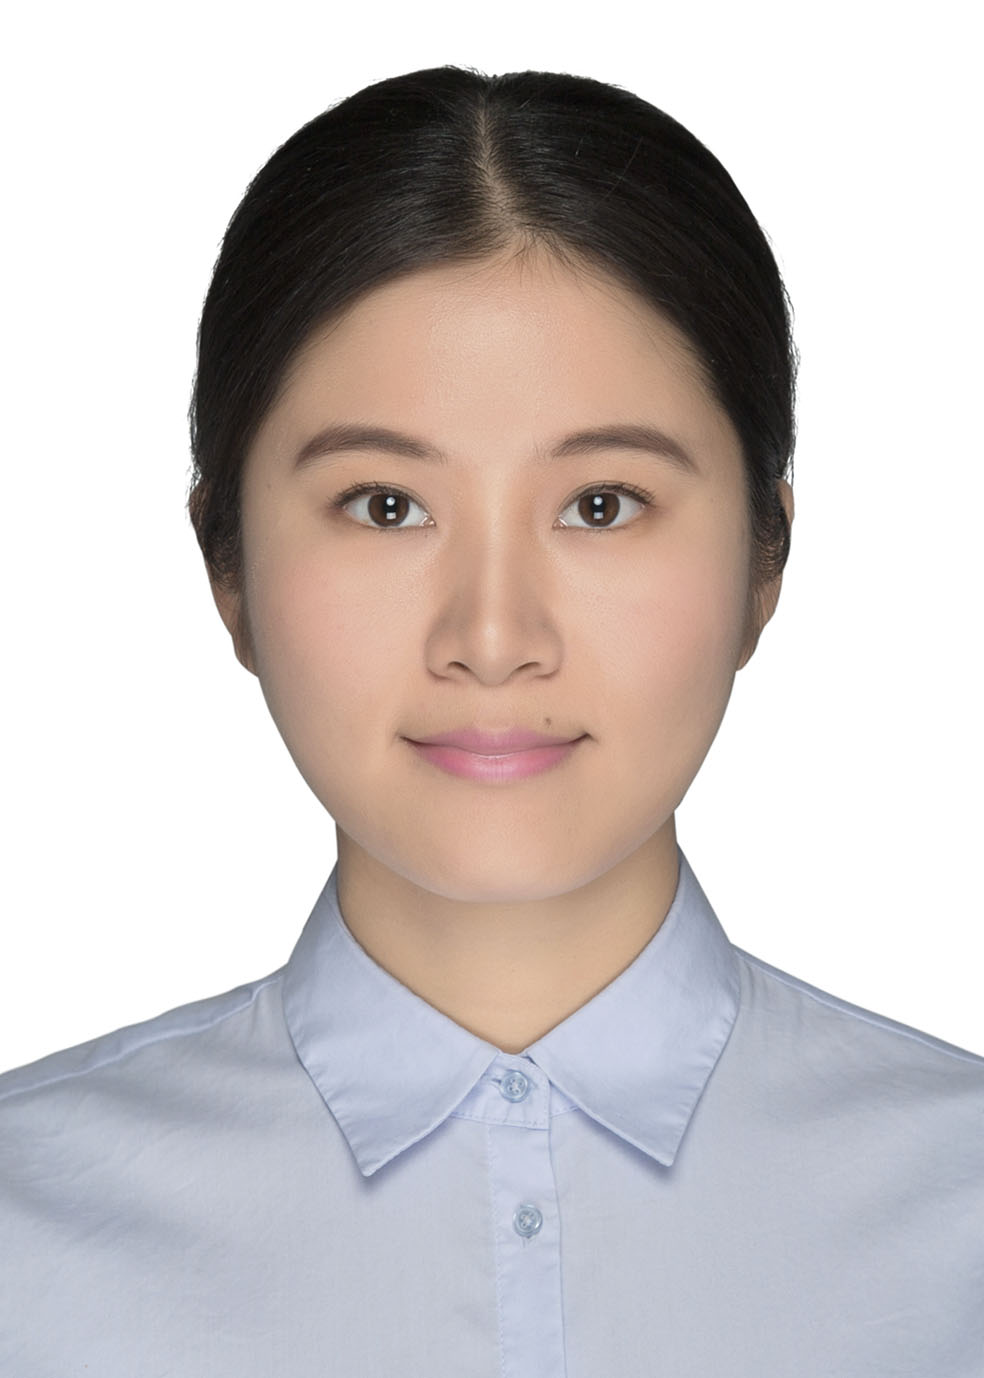
\includegraphics[width=0.8in,height=1in,clip,keepaspectratio]{photos/jie.jpg}}]{Jie Zhu} is currently studying for Master degree of Computer Science in Graduate School at Shenzhen, Tsinghua University. She received her Bachelor degree in Beijing University of Posts and Telecommunications. Her current research interests include verifiable data search and privacy.
\end{IEEEbiography}

\vspace{-5.5em}

\begin{IEEEbiography}[{\vspace{-1em}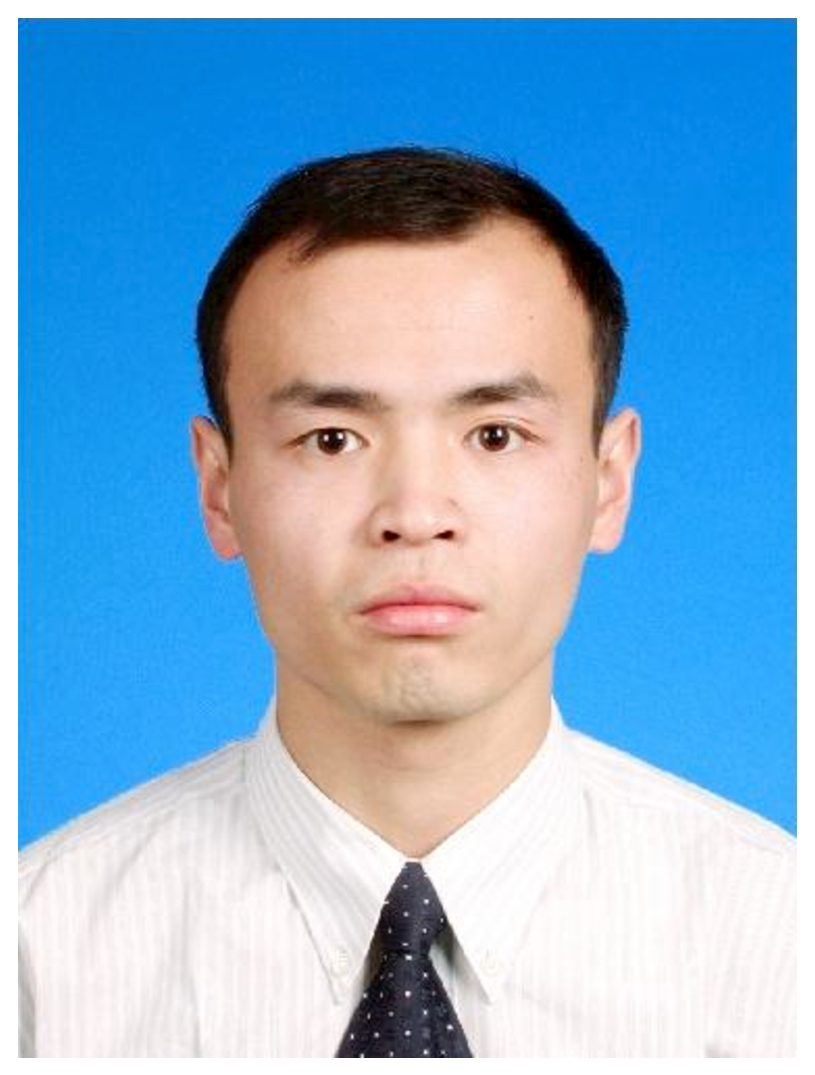
\includegraphics[width=0.8in,height=1in,clip,keepaspectratio]{photos/qi.eps}}]{Qi Li} received his Ph.D. degree from Tsinghua University. Now he is an associate professor of Graduate School at Shenzhen, Tsinghua University. He has ever worked at ETH Zurich, the University of Texas at San Antonio, The Chinese University of Hong Kong, Chinese Academy of Sciences, and Intel.
His research interests are in network and system security, particularly in Internet and cloud security, mobile security, and big data security. He is currently an editorial board member of IEEE TDSC.%, and has served on the organization or program committees of numerous conferences.
\end{IEEEbiography}

\vspace{-3.5em}

\begin{IEEEbiography}[{\vspace{-1em}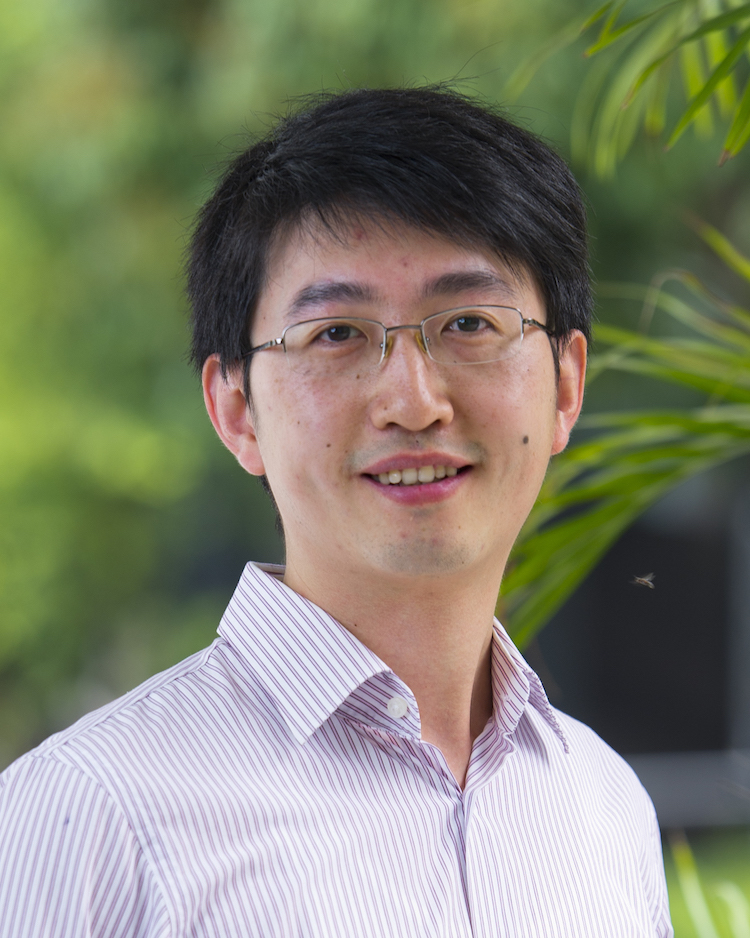
\includegraphics[width=0.8in,height=1in,clip,keepaspectratio]{photos/cong.jpeg}}]{Cong Wang} received the PhD degree in electrical and computer engineering from the Illinois Institute of Technology, in 2012. He is an assistant professor in the Computer Science Department, City University of Hong Kong. He worked at the Palo Alto Research Center in the summer of 2011. His research interests include the areas of cloud computing security, with current focus on secure data outsourcing and secure computation outsourcing in public cloud.
\end{IEEEbiography}

\vspace{-3.5em}
\begin{IEEEbiography}[{\vspace{-1em}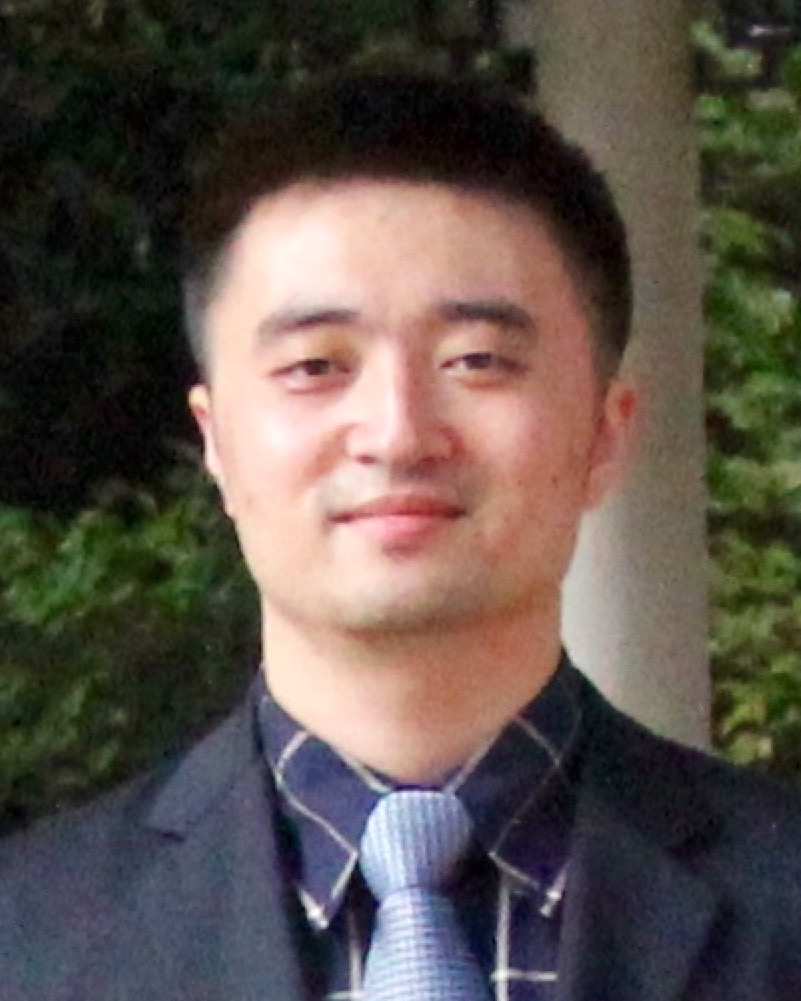
\includegraphics[width=0.8in,height=1in,clip,keepaspectratio]{photos/yuan.jpg}}]{Xingliang Yuan} received the B.S. degree from Nanjing University of Posts and Telecommunications in 2008, the M.S. degree from Illinois Institute of Technology in 2009, both in Electrical Engineering, and the Ph.D. degree in Computer Science from City University of Hong Kong in 2016. He is a Lecturer with the Faculty of Information Technology at Monash University. His research interests include cloud security, NFV security, and privacy-aware computing.
\end{IEEEbiography}

\vspace{-3.5em}

%\vspace{-30em}
\begin{IEEEbiography}[{\vspace{-1em}\includegraphics[width=0.8in,height=1in,clip,keepaspectratio]{photos/qian.eps}}]{Qian Wang} received the B.S. degree from Wuhan University, Wuhan, China, in 2003, the M.S. degree from Shanghai Institute of Microsystem and Information Technology (SIMIT), Chinese Academy of Sciences, Shanghai, China, in 2006, and the Ph.D. degree from Illinois Institute of Technology, Chicago, IL, USA, in 2012, all in electrical engineering.He is a Professor with the School of Computer Science, Wuhan University. His research interests include wireless network security and privacy, cloud computing security, and applied cryptography. He is currently an editorial board member of IEEE TIFS.
\end{IEEEbiography}

\vspace{-3.5em}

\begin{IEEEbiography}[{\vspace{-1em}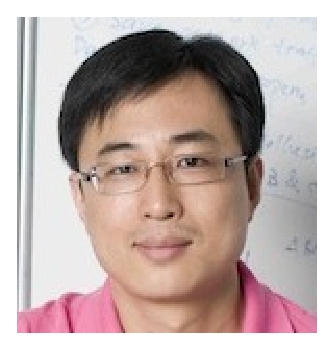
\includegraphics[width=0.8in,height=1in,clip,keepaspectratio]{photos/kuiren.eps}}]{Kui Ren} received the Ph.D. degree from the Worcester Polytechnic Institute. He is currently a Professor of Institute of Cyber Security Research in Zhejiang University. His current research interests span cloud and outsourcing security, wireless and wearable system security, and human-centered computing. He currently serves as an Associate Editor of IEEE TDSC, TMC, IEEE TSG, IEEE Wireless Communications, IEEE IoT Journal, Pervasive and Mobile Computing (Elsevier), and The Computer Journal (Oxford).


%He currently serves as an Associate Editor of various premier journals, e.g., IEEE TMC, IEEE TDSC.  %e.g., the IEEE Transactions on Dependable and Secure Computing and the IEEE Transactions on Mobile Computing.
%He was a recipient of the NSF CAREER Award in 2011 and the Sigma Xi/IIT Research Excellence Award in 2012. He has authored 135 peer-reviewed journal and conference papers and received several best paper awards, including the IEEE ICNP 2011.
%He currently serves as an Associate Editor of the IEEE Transactions on Dependable and Secure Computing, the IEEE Transactions on Mobile Computing, the IEEE Wireless Communications, the IEEE Internet of Things Journal, the IEEE Transactions on Smart Grid, Pervasive and Mobile Computing (Elsevier), and The Computer Journal (Oxford).
\end{IEEEbiography}


%\appendices
%\section{}
%Appendix one text goes here.

% you can choose not to have a title for an appendix
% if you want by leaving the argument blank


% use section* for acknowledgment
%\ifCLASSOPTIONcompsoc
  % The Computer Society usually uses the plural form
%  \section*{Acknowledgments}
%\else
  % regular IEEE prefers the singular form
%  \section*{Acknowledgment}
%\fi



% Can use something like this to put references on a page
% by themselves when using endfloat and the captionsoff option.
%\ifCLASSOPTIONcaptionsoff
%  \newpage
%\fi


%\begin{IEEEbiography}{Jie Zhu}
%Biography text here.
%\end{IEEEbiography}

%\renewcommand\refname{Reference}
%\bibliographystyle{plain}
%\bibliography{Reference}



% that's all folks
\end{document}
